% !TEX program = xelatex
% !TEX option = -shell-escape
% Generated by tools/build_latex.py; edit chapter fragments, not Markdown.
\documentclass[bwprint]{gmcmthesis}
\geometry{top=25mm,bottom=25mm,left=25mm,right=25mm,headsep=15mm}
\renewcommand{\baselinestretch}{1.0}
\normalsize
\def\GMCMEvaluationSection{7}
\hypersetup{hidelinks}
\renewcommand{\thesubsection}{\arabic{section}.\arabic{subsection}}
\renewcommand{\thesubsubsection}{\thesubsection.\arabic{subsubsection}}
\pagestyle{plain}
\usepackage[framemethod=TikZ]{mdframed}
\usepackage{subfig}
\usepackage{siunitx}
\usepackage{colortbl}
\usepackage{array}
\usepackage{tabularx}
\usepackage{longtable}
\AtEndEnvironment{thebibliography}{\bibitem{ai_tool_disclosure}DeepSeek，DeepSeek-V4.1-Flash，深度求索（DeepSeek），2026-09-23。}
% 华为杯统一附录模板。
% 本文件由 build_latex.py 复制到论文目录并在导言区实际 \input；
% 生成内容只能调用这里的接口，不得在章节片段中另设代码样式。
\usepackage{minted}
\usepackage{xcolor}
\usepackage{tcolorbox}
\tcbuselibrary{breakable,skins}
\usepackage{longtable}
\usepackage{booktabs}
\usepackage{array}
\usepackage{needspace}
\usemintedstyle{lovelace}

% 克制的浅色学术代码配色。语法 token 由 Pygments 的 lovelace 浅色主题生成；
% 下列颜色只负责纸面、边线和行号，不覆盖 Pygments token 语义。
\definecolor{AppendixStripeWhite}{HTML}{FFFFFF}
\definecolor{AppendixStripeGray}{HTML}{F8F8F8}
\definecolor{AppendixDivider}{HTML}{63B96C}
\definecolor{AppendixHorizontalRule}{HTML}{555B57}
\definecolor{AppendixLineNumber}{HTML}{6F8175}
\definecolor{AppendixCaption}{HTML}{343A36}
\newfontfamily\AppendixCodeLatin{Consolas}[Scale=MatchLowercase]
\newcommand{\AppendixCodeFont}{\songti\AppendixCodeLatin}
\renewcommand{\myFont}{\AppendixCodeFont}

% Pygments 仍负责词法分类；在 lovelace 浅色基底上将论文要求的
% “关键词紫、字符串绿、数字/类型棕橙、注释灰绿”固化为低饱和调色板。
% Minted 在首次代码块前载入 Pygments style，因此在 MintedVerbatim
% 开始时覆写 token 显示色，避免被后载入的 styledef 反向覆盖。
\makeatletter
\newcommand{\AppendixPygmentsPalette}{%
  \@namedef{PYG@tok@k}{\def\PYG@tc####1{\textcolor[HTML]{8B4E8F}{####1}}}%
  \@namedef{PYG@tok@kc}{\def\PYG@tc####1{\textcolor[HTML]{8B4E8F}{####1}}}%
  \@namedef{PYG@tok@kd}{\def\PYG@tc####1{\textcolor[HTML]{8B4E8F}{####1}}}%
  \@namedef{PYG@tok@kn}{\def\PYG@tc####1{\textcolor[HTML]{8B4E8F}{####1}}}%
  \@namedef{PYG@tok@kp}{\def\PYG@tc####1{\textcolor[HTML]{8B4E8F}{####1}}}%
  \@namedef{PYG@tok@kr}{\def\PYG@tc####1{\textcolor[HTML]{8B4E8F}{####1}}}%
  \@namedef{PYG@tok@kt}{\def\PYG@tc####1{\textcolor[HTML]{8B4E8F}{####1}}}%
  \@namedef{PYG@tok@ow}{\def\PYG@tc####1{\textcolor[HTML]{8B4E8F}{####1}}}%
  \@namedef{PYG@tok@s}{\def\PYG@tc####1{\textcolor[HTML]{4F8A55}{####1}}}%
  \@namedef{PYG@tok@s1}{\def\PYG@tc####1{\textcolor[HTML]{4F8A55}{####1}}}%
  \@namedef{PYG@tok@s2}{\def\PYG@tc####1{\textcolor[HTML]{4F8A55}{####1}}}%
  \@namedef{PYG@tok@sa}{\def\PYG@tc####1{\textcolor[HTML]{4F8A55}{####1}}}%
  \@namedef{PYG@tok@sd}{\def\PYG@tc####1{\textcolor[HTML]{4F8A55}{####1}}}%
  \@namedef{PYG@tok@si}{\def\PYG@tc####1{\textcolor[HTML]{4F8A55}{####1}}}%
  \@namedef{PYG@tok@m}{\def\PYG@tc####1{\textcolor[HTML]{A06D20}{####1}}}%
  \@namedef{PYG@tok@mi}{\def\PYG@tc####1{\textcolor[HTML]{A06D20}{####1}}}%
  \@namedef{PYG@tok@mf}{\def\PYG@tc####1{\textcolor[HTML]{A06D20}{####1}}}%
  \@namedef{PYG@tok@mh}{\def\PYG@tc####1{\textcolor[HTML]{A06D20}{####1}}}%
  \@namedef{PYG@tok@mo}{\def\PYG@tc####1{\textcolor[HTML]{A06D20}{####1}}}%
  \@namedef{PYG@tok@nb}{\def\PYG@tc####1{\textcolor[HTML]{9A702D}{####1}}}%
  \@namedef{PYG@tok@c}{\def\PYG@tc####1{\textcolor[HTML]{7A887E}{####1}}}%
  \@namedef{PYG@tok@c1}{\def\PYG@tc####1{\textcolor[HTML]{7A887E}{####1}}}%
  \@namedef{PYG@tok@cm}{\def\PYG@tc####1{\textcolor[HTML]{7A887E}{####1}}}%
  \@namedef{PYG@tok@cp}{\def\PYG@tc####1{\textcolor[HTML]{6F8175}{####1}}}%
}
% 用 fvextra 的全宽行盒绘制白/极浅灰逻辑行底纹。breaklines 产生的
% 视觉续行仍位于同一个 parbox 中，因此保持与源代码逻辑行相同的底色。
\newcommand{\AppendixFullWidthStripe}[2]{%
  \setlength{\FV@TmpLength}{\fboxsep}%
  \setlength{\fboxsep}{0pt}%
  \colorbox{#1}{%
    \setlength{\fboxsep}{\FV@TmpLength}%
    \rlap{\strut#2}%
    \hspace{\linewidth}%
    \ifx\FV@RightListFrame\relax\else
      \hspace{-\FV@FrameSep}\hspace{-\FV@FrameRule}%
    \fi
    \ifx\FV@LeftListFrame\relax\else
      \hspace{-\FV@FrameSep}\hspace{-\FV@FrameRule}%
    \fi
  }%
  \hss
}
\newcommand{\AppendixZebraLine}[1]{%
  \ifodd\value{FancyVerbLine}%
    \AppendixFullWidthStripe{AppendixStripeWhite}{#1}%
  \else
    \AppendixFullWidthStripe{AppendixStripeGray}{#1}%
  \fi
}
\AtBeginEnvironment{MintedVerbatim}{\AppendixPygmentsPalette}
\makeatother

% 透明、无左右框的可分页外壳。overlay 会在 unbroken/first/middle/last
% 每个物理分片上执行，从而显式重复绘制上下细横线。
\newtcolorbox{AppendixCodePageFrame}{%
  enhanced jigsaw,
  breakable,
  width=\linewidth,
  colback=white,
  colframe=AppendixHorizontalRule,
  boxrule=0pt,
  leftrule=0pt,
  rightrule=0pt,
  toprule=0pt,
  bottomrule=0pt,
  boxsep=0pt,
  left=0pt,
  right=0pt,
  % 为每个物理分页片段的横线保留极窄的无遮挡带，避免首/末行
  % 的全宽 zebra 色块覆盖横线主体。
  top=1.5pt,
  bottom=1.5pt,
  arc=0pt,
  outer arc=0pt,
  sharp corners,
  before skip=0.15\baselineskip,
  after skip=0.20\baselineskip,
  lines before break=3,
  overlay={%
    \draw[AppendixHorizontalRule,line width=0.5pt]
      ([yshift=-0.25pt]frame.north west)--([yshift=-0.25pt]frame.north east);%
    \draw[AppendixHorizontalRule,line width=0.5pt]
      ([yshift=0.25pt]frame.south west)--([yshift=0.25pt]frame.south east);%
  }
}

\setminted{
  encoding=utf8,
  linenos,
  numberblanklines=true,
  numbersep=6pt,
  breaklines,
  breakanywhere,
  autogobble,
  tabsize=4,
  obeytabs=true,
  fontfamily=myFont,
  fontsize=\fontsize{10.2pt}{13.5pt}\selectfont,
  baselinestretch=1.0,
  frame=leftline,
  framesep=5pt,
  framerule=0.55pt,
  rulecolor=\color{AppendixDivider},
  xleftmargin=3.15em,
  xrightmargin=0pt,
  listparameters={\setlength{\topsep}{0pt}\setlength{\partopsep}{0pt}\setlength{\parsep}{0pt}},
  resetmargins=true,
  style=lovelace
}

\newcommand{\AppendixStart}{%
  \section{附录}%
}

\newcommand{\AppendixPart}[2]{%
  \par\vspace{1.3\baselineskip}%
  \phantomsection
  \noindent{\songti\fontsize{12pt}{18pt}\selectfont\bfseries 附录 #1：#2}\par
  \addcontentsline{toc}{subsection}{附录 #1：#2}%
  \vspace{0.55\baselineskip}%
}

\newcommand{\AppendixAttachmentTableBegin}{%
  \begingroup
  \renewcommand{\arraystretch}{1.18}%
  \setlength{\tabcolsep}{4pt}%
  \small
  \begin{longtable}{>{\centering\arraybackslash}p{1.0cm}p{3.0cm}p{10.0cm}}
  \toprule
  序号 & 文件夹名称 & 主要内容 \\
  \midrule
  \endfirsthead
  \toprule
  序号 & 文件夹名称 & 主要内容 \\
  \midrule
  \endhead
  \midrule
  \multicolumn{3}{r}{续下页}\\
  \endfoot
  \bottomrule
  \endlastfoot
}

\newcommand{\AppendixAttachmentRow}[3]{%
  #1 & #2 & #3 \\
}

\newcommand{\AppendixAttachmentTableEnd}{%
  \end{longtable}
  \endgroup
}

% #1: 可选 minted 参数（支持 firstline/lastline/firstnumber）
% #2: 代码片段标题；#3: Pygments lexer；#4: 真实源码路径。
\newcommand{\AppendixCodeFile}[4][]{%
  \Needspace{6\baselineskip}%
  \par\vspace{0.35\baselineskip}%
  \noindent{\color{AppendixCaption}\songti\fontsize{10.5pt}{15pt}\selectfont #2}\par
  \vspace{0.15\baselineskip}%
  \begingroup
  \renewcommand{\theFancyVerbLine}{\AppendixCodeLatin\fontsize{8.6pt}{13.5pt}\selectfont\color{AppendixLineNumber}\arabic{FancyVerbLine}}%
  \let\FancyVerbHighlightLine\AppendixZebraLine
  \begin{AppendixCodePageFrame}%
    \inputminted[#1]{#3}{#4}%
  \end{AppendixCodePageFrame}%
  \endgroup
  \par\vspace{0.25\baselineskip}%
}

\newcommand{\AppendixEnd}{\par}

\newcommand{\codeid}[1]{\nolinkurl{#1}}
\usepackage{booktabs}
\usepackage{tikz}
\usetikzlibrary{arrows.meta,positioning,fit,calc,shapes.geometric,shapes.arrows}
\makeatletter
\newcommand{\HuaweiLabel}[1]{{\lishu\fontsize{18pt}{24pt}\selectfont #1}}
\newcommand{\HuaweiBodyFont}{\songti\fontsize{12pt}{18pt}\selectfont}
\newcommand{\HuaweiTitleUnderline}[1]{%
  \begingroup
  \renewcommand{\ULthickness}{1.2pt}%
  \setlength{\ULdepth}{4pt}%
  \uline{#1}%
  \endgroup
}
\newcommand{\HuaweiPaperTitle}[1]{%
  \begin{minipage}[t]{.9\textwidth}\centering
    \HuaweiLabel{题\quad 目：}\hspace{0.4em}{\zihao{3}\heiti #1}%
  \end{minipage}%
}
\newcommand{\HuaweiTitlePage}{%
  \clearpage\thispagestyle{plain}\setcounter{page}{1}%
  \GMCMContestTitle{二十三}
  \vspace{8mm}\noindent
  \begin{center}
    \HuaweiPaperTitle{\HuaweiTitleUnderline{通用神经网络处理器下的多核调度问题}}
  \end{center}
  \vspace{3mm}
}
\renewenvironment{abstract}{%
  \begin{center}\GMCMAbstractHeading\end{center}\HuaweiBodyFont\quotation
}{%
  \endquotation\clearpage
}
\renewcommand{\keywords}[1]{\par\vspace{1ex}{\noindent\HuaweiLabel{关键词：}}~{\HuaweiBodyFont #1}\par}
\makeatother
\title{通用神经网络处理器下的多核调度问题}

\begin{document}
\HuaweiTitlePage
\begin{abstract}
本文针对通用神经网络处理器上依赖图切分、同核任务合并与共享只读缓存联动的多核调度问题，建立从合法方案构造到官方事件评估的统一模型，依据操作—张量依赖、私有存储容量、跨核同步和共享带宽约束，采用有限候选划分与逐例成对比较，得到题定配置下最高的五核平均加速比\textbf{3.6104（无量纲）}。研究以全局完成周期最小化为目标。三个场景均覆盖全部官方算例和一至五核配置，结果同时保留分位分布、候选差异与时间线核验，以避免仅凭局部负载或单一搬运量解释全局性能。

\textbf{针对问题一}，场景A规定每个子图是独立Task，私有缓存不能跨Task沿用，因而切分过细会增加DDR中转与固定等待。建立操作覆盖、收缩依赖无环及同核顺序相容的调度模型，以官方全局Makespan为目标函数，约束核心编号、子图划分和任务先后。采用\textbf{连通块分核}，并与依赖深度分段、宽图分批两个候选比较；每个候选先过合法性校验，再使用未改动的官方评估器择优。得到五核平均加速比\textbf{3.5093（无量纲）}，其分位范围与结构分层共同表明\textbf{多数图可利用多个核心}，但大块占优或新增传输较高的图保留低加速尾部。独立重算后，所选五百组方案的覆盖、时间线及官方响应交叉核验全部通过；逐例结果仍显示增核不必然单调加速。

\textbf{针对问题二}，基于问题一的合法切图，在场景B中把同核子图合并为Task，使中间张量可留在L1或UB，同时承担容量压力与可能的Spill。建立场景B调度模型，沿用全局周期最小化目标，并引入逐时刻私有存储容量、跨核边界COPY及固定同步约束，采用\textbf{场景B重新择优}，并把问题一选中方案直接放入B作同方案A/B对照，以分开硬件规则和方案选择的收益。得到五核平均加速比\textbf{3.5456（无量纲）}；成对时长比的逐例范围揭示\textbf{Task合并并不保证逐例加速}，其原因可能是驻留量、Spill与共享DDR争用共同改变关键路径。独立重算后，所选五百组方案的覆盖、时间线及官方响应交叉核验全部通过，容量峰值和新增搬运分解按官方详细输出逐例对照。

\textbf{针对问题三}，进一步在场景B中引入按逻辑张量编号查询的共享只读L2；命中与未命中分别竞争Cache读池和DDR读池，FIFO次序与容量影响后续复用。建立两读池、缓存状态与依赖事件共同决定Makespan的调度模型，以全局周期最小化为目标，并约束只在输入搬运事件使用L2。采用\textbf{同方案反事实}比较题定缓存开关，得到五核平均加速比\textbf{3.6104（无量纲）}及同方案缓存时长比均值\textbf{1.0260（无量纲）}；\textbf{有正向收益的算例过半}，但命中字节率不能直接等同于完成时间收益。所选五百组方案的覆盖、时间线及官方响应交叉核验全部通过；另在六个有代表性的案例上改变容量和带宽，独立验证默认格与正式结果一致，并将该网格明确作为机制敏感性分析。

创新点在于先保持切图更换Task语义、再保持方案单独切换L2读路径；相比只报告各场景最终方案的速度，成对设计另以\textbf{1.0260（无量纲）}的五核同方案Cache比度量缓存机制效果。


\keywords{多核调度\quad 有向无环图\quad 子图划分\quad 共享缓存\quad 离散事件评估}
\end{abstract}
\setcounter{tocdepth}{3}
\clearpage
\maketoc
\clearpage
\HuaweiBodyFont
\section{问题重述}
\subsection{问题背景}

待调度的对象是由操作节点和张量节点交替连接而成的有向无环计算图。操作表示一次计算或数据搬运，张量表示其输入、中间结果或输出；两者之间的有向边规定了操作何时才能开始。对于分块神经网络计算，一个计算块可能先由外部存储器搬入核内，再由矩阵或向量单元处理，最后将结果写回外部存储器。多个块的依赖、共享输入和中间张量驻留同时存在，因此仅按操作数平均分配到各核，不能保证总完成时间缩短。

神经网络处理器研究已有对硬件平台、体系结构及降低计算成本路径的系统综述\cite{sze2017}。Eyeriss 对局部复用和片外访存能耗的实证分析说明，数据流设计会显著改变搬运代价\cite{eyeriss2017}；TPU 的整模型评估则提醒我们，专用矩阵单元的峰值能力不能单独代表应用完成时间\cite{jouppi2017}。经典的红蓝卵石模型从理论上刻画有限快存下计算与I/O的牵制\cite{hongkung1981}。这些研究提供背景，本题的数值结果仍以题给评估语义为准。

题目给定的平台由若干同构 NPU 核心及共享 DDR 组成。每个核心具备矩阵、向量和两类数据搬运流水线，同时有私有 L1 与 UB 缓存；各核的 DDR 读写争用同一物理带宽。跨核并行可分担计算，但张量一旦跨越不能直接复用的边界，就可能增加读写与同步等待。反过来，过度合并虽然减少边界，却会拉长单个核心的计算段，并使中间张量占据缓存更久。切图、分核和核内顺序由此相互牵制。

这种牵制还取决于硬件组织。无核间同步机制时，每个子图作为单独 Task 下发，同核相邻 Task 也不能保留前一 Task 的私有缓存；有同步机制时，同核多个子图可合成一个 Task，保留部分中间数据，但跨核张量仍需经 DDR 中转。后者可能节省边界读写，也可能让长时间驻留的张量挤占缓存。进一步引入共享只读 L2 后，多核重复读取的部分输入有机会改由 Cache 服务，而命中率又受容量、FIFO 淘汰顺序和读带宽约束。这三种条件需要按各自真实规则评价。

本题提供完整计算图、容量与带宽配置、合法方案格式，以及包含核内排布和多核事件模拟的评估程序。评估程序会根据子图边界补充搬运、在必要时插入缓存换入换出，并在共享带宽争用下重算全局操作完成时刻。因此，单独的拓扑层数、各核工作量总和或核内参考时间都不能直接充当最终 Makespan。研究需要同时保证方案覆盖与依赖合法、私有存储不越界、全局执行能结束，并在相同的官方配置下比较总时长和新增搬运量。

\subsection{问题重述}

对每个给定计算图，需要把全部非 COPY 操作映射到子图编号，把每个子图恰好安排到一个核心，并给出同核子图的执行顺序。子图依赖图不得有环，顺序不得违反依赖；方案交由题目规定的评估流程确定核内操作序、缓存换入换出和共享资源上的实际时间线。核心数量变化时，方法仍应在合理时间内产生可执行方案。评价以全局 Makespan 为主，同时控制相对原始图增加的 DDR 搬运字节数。

问题一针对场景 A：一个子图就是一个 Task，跨子图张量都须经 DDR；跨核前驱 Task 与同核 Task 切换分别受题定等待时间约束。应建立切图和调度模型，分别为二至五核生成方案。正文需展示以整图单核时长为基准的一至五核平均加速比，逐例结果表列出全部给定算例的官方 Makespan 与额外搬运量，并保留可复现程序和方案文件。

问题二针对场景 B：同核全部子图合为一个 Task，可在 L1 或 UB 中复用数据，跨核依赖则以 DDR 拷贝和固定同步延迟实现。需在满足每核私有缓存容量的前提下，调整切图、分核与顺序，在二至五核稳定生成方案，争取进一步降低全局时长和额外搬运。其平均加速比仍以与问题一相同的整图单核结果为分母；逐例指标与方案同样须保留在支撑材料中，并提供可复现的 Python 程序。

问题三在场景 B 上增加所有核心共享的只读 L2。只有 COPY\_IN 查询 Cache；命中不改变 FIFO 顺序，L2 读带宽与 DDR 带宽独立。需研究容量与读带宽变化如何影响切图、调度及完成时间，设计相应方案，并在题定容量和带宽下完成全部正式用例。正文比较同核数无 L2 与有 L2 的结果，Cache 加速比须在同一方案上用无 L2 时长除以有 L2 时长；逐例结果表列出两种配置的 Makespan、额外搬运量和命中率。

本文的研究安排如图~\ref{fig:roadmap} 所示。

\begin{figure}[htbp]
  \centering
  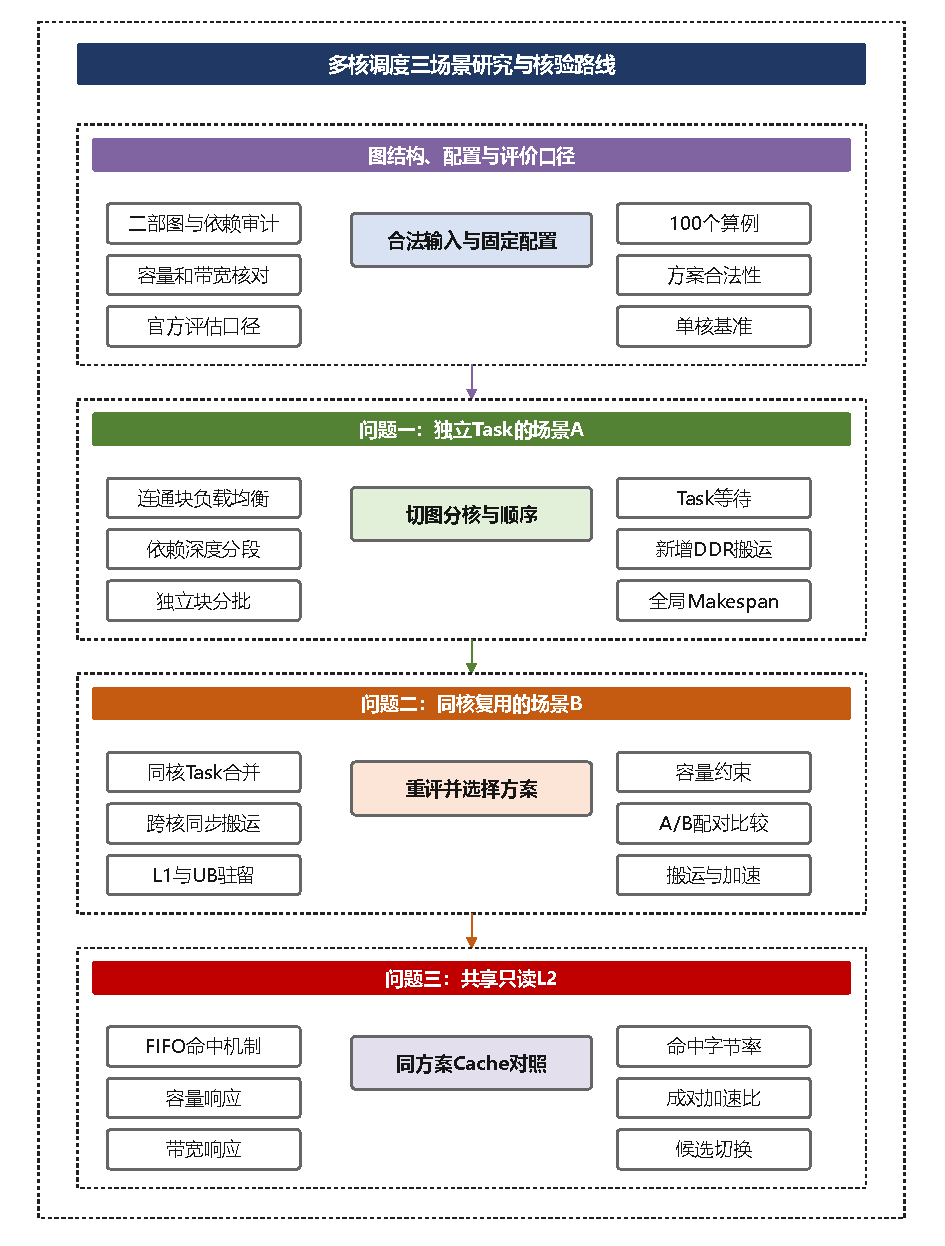
\includegraphics[width=160mm]{../求解/总体路线图_论文宽.pdf}
  \caption{多核调度研究路线}
  \label{fig:roadmap}
\end{figure}

\FloatBarrier

路线图先核查图结构、配置及评估口径，再依照场景 A、场景 B 和共享 L2 的条件组织候选方案与合法性验证，最后用同一批官方算例比较速度、搬运和缓存响应。这一路线是本文的求解安排，并不改变题目对三个问题的交付要求。



\GMCMChapterEnd{1}
\section{模型假设}

题定的计算图、操作周期、缓存容量、总带宽及场景等待规则均作为固定输入；最终时长由官方确定性模拟器给出，不把这些题定条件另称为假设。为把不可直接枚举的切图与调度组合收敛到可计算的候选集合，本文只在构造方案时采用以下工作假设。

其一，把非 COPY 操作的给定计算周期加一个固定单位作为连通块的粗略负载权重。该权重只用于决定连通块向核心的初始分配，不预言实际运行时间；加一避免零周期操作在排序中完全失重。由于不同流水线可重叠、DDR 搬运会争用，这一代理可能低估通信密集块的代价，因而最终选择必须重新使用官方全局评估。

其二，把收缩 COPY 后互无依赖的弱连通块视为可独立分配的基本单元。这里的“独立”仅指该收缩图中没有非 COPY 操作依赖，并不假定它们在共享 DDR 上互不干扰。对于存在较大连通块的图，允许再沿拓扑深度切分；由此产生的跨段边界须由官方规则插入搬运并验证无环。

其三，候选搜索采用确定性排序与固定的规模阈值，同分时按操作编号或核心编号打破并列。这保证相同输入重复运行得到相同方案。候选集合不是全局最优解的证明；保留多个不同粒度的方案并按官方 Makespan 比较，同时用额外搬运量处理同等时长的取舍。共享 L2 研究还需把同一方案在有、无 L2 两种条件下成对评估，避免把方案变化误当作 Cache 效益。

\GMCMChapterEnd{2}
\section{关键性符号说明}

下表汇集贯穿三个问题的对象、容量及评价量；局部启发式参数在首次使用处说明。
\begin{GMCMSymbolTable}{符号中 $i$ 表示操作，$j$ 表示张量，$k$ 表示核心数。}
\GMCMSymbolRow{集合}{G}{输入的有向无环二部计算图}{—}
\GMCMSymbolRow{集合}{\mathcal{O}}{计算图中的操作节点集合}{—}
\GMCMSymbolRow{集合}{\mathcal{T}}{计算图中的张量节点集合}{—}
\GMCMSymbolRow{集合}{E}{计算图的有向依赖边集合}{—}
\GMCMSymbolRow{索引}{i}{操作节点的索引}{1}
\GMCMSymbolRow{索引}{j}{张量节点的索引}{1}
\GMCMSymbolRow{索引}{k}{参与调度的核心数}{1}
\GMCMSymbolRow{参数}{c_i}{操作 $i$ 的题定计算周期}{cycle}
\GMCMSymbolRow{参数}{s_j}{张量 $j$ 占用的字节数}{byte}
\GMCMSymbolRow{变量}{g(i)}{非 COPY 操作 $i$ 所属的子图编号}{1}
\GMCMSymbolRow{变量}{a(g)}{子图 $g$ 被分配的核心编号}{1}
\GMCMSymbolRow{参数}{C_{\mathrm{L1}}}{每个核心的 L1 容量}{byte}
\GMCMSymbolRow{参数}{C_{\mathrm{UB}}}{每个核心的 UB 容量}{byte}
\GMCMSymbolRow{参数}{B_{\mathrm{DDR}}}{全部核心共享的 DDR 总带宽}{byte/cycle}
\GMCMSymbolRow{参数}{C_{\mathrm{L2}}}{共享只读 L2 容量}{byte}
\GMCMSymbolRow{参数}{B_{\mathrm{L2}}}{共享只读 L2 读带宽}{byte/cycle}
\GMCMSymbolRow{指标}{T_k}{$k$ 核方案的全局 Makespan}{cycle}
\GMCMSymbolRow{指标}{T_1}{原始整图单核基准 Makespan}{cycle}
\GMCMSymbolRow{指标}{S_k}{相对于整图单核基准的加速比}{1}
\GMCMSymbolRow{指标}{D_k}{相对原图新增的 DDR 搬运量}{byte}
\GMCMSymbolRow{指标}{H_k}{可由 L2 服务的 COPY\_IN 字节命中率}{1}
\end{GMCMSymbolTable}


\GMCMChapterEnd{3}
\section{问题一求解与分析}
\subsection{问题的描述与分析}

场景 A 把每个子图作为独立 Task。即使两个相邻 Task 被安排到同一核心，前一 Task 的私有缓存也不再可用；跨子图张量须由 DDR 中转。同核顺序和跨核前驱分别触发不同的固定等待，因此切图粒度本身会改变调度开销。过粗的子图压缩并行度，过细的子图增加 Task 切换及搬运。图~\ref{fig:q1-overview} 将计算图、依赖约束、候选切图及官方核验放在一条研究链中，具体统计图在本章结果段给出。

% Generated figure only; description and reference belong before this input.
\begin{figure}[!htbp]
\centering
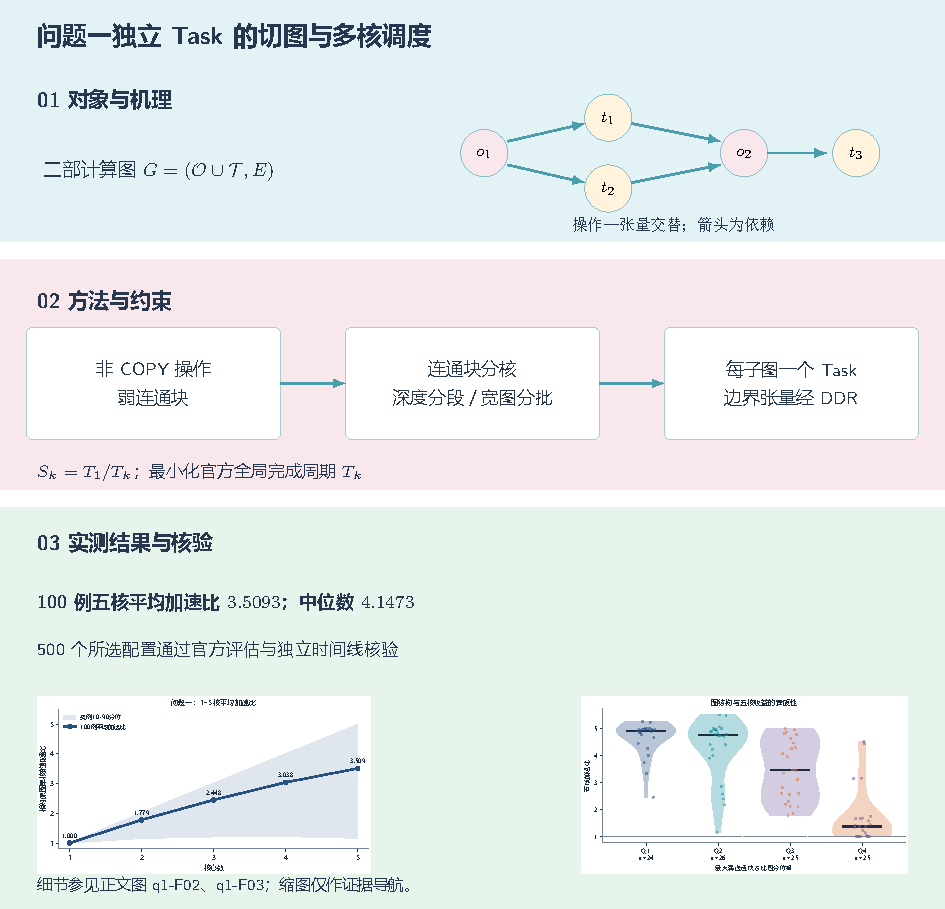
\includegraphics[width=160mm]{../求解/综合图/q1-overview.pdf}
\caption{问题一求解与核验总览}\label{fig:q1-overview}
\end{figure}
\FloatBarrier


多资源列表调度研究把核心、缓存、内存和I/O与任务先后约束共同纳入完工时间目标\cite{perotin2021}；针对有向无环任务图的HEFT算法还把执行代价和通信代价共同用于任务排序\cite{topcuoglu2002}。Kernighan--Lin以给定规模限制下的割边代价为划分目标\cite{kernighan1970}；多层次方法则通过粗化、粗图划分和细化逐步改善割边\cite{karypis1998}。本题同时存在Task切换、私有存储和共享DDR竞争，因此这些算法在本文作为建模参照，最终分数仍由题定评估器给出。

\subsection{切图与调度模型}

记输入二部图为 $G$，并写成 $G=(\mathcal{O}\cup\mathcal{T},E)$。$\mathcal{O}$ 是操作节点集合，$\mathcal{T}$ 是张量节点集合，$E$ 仅连接不同类型节点。对每个非 COPY 操作 $i$ 定义子图编号 $g(i)$；对子图 $g$ 定义核心编号 $a(g)$，并令每核子图序列形成一个全排列。所有非 COPY 操作必须且只能出现一次，子图依赖收缩图必须无环，同核序列须与该图的偏序相容。这些是硬约束，并在正式计分前由题目提供的校验程序执行。

对核数 $k$，令官方评估程序得到的全局完成时间为 $T_k$，原始整图单核完成时间为 $T_1$，则本题要求的加速比 $S_k$ 为
\begin{equation}\label{eq:q1-speedup}
S_k=\frac{T_1}{T_k},\qquad S_1=1.
\end{equation}
令 $D_k$ 为调度后 DDR 搬运字节数减去原图已有的搬运字节数。方案选择以最小化 $T_k$ 为第一目标；相同完成时间时，优先较小的 $D_k$。这里的 $T_k$ 是四条 Pipe、私有缓存、Task 等待与共享 DDR 带宽共同作用后的事件模拟结果，不用任何核内局部排布时间替代。

\subsection{候选构造与合法性}

采用连通块分核，先按官方图转换规则消去 COPY 端点，在非 COPY 操作上建立收缩依赖 DAG。该操作保留通过 COPY 链连接的先后关系。对其无向弱连通块，若两个操作落在不同块，就不存在块间非 COPY 依赖。连通块因此可以独立分核；块内部保持完整，避免直接切断其依赖。设块 $C$ 的粗负载为
\begin{equation}\label{eq:q1-load}
w(C)=\sum_{i\in C}(c_i+1),
\end{equation}
其中 $c_i$ 为题定计算周期。按 $w(C)$ 递减排序，把下一个块分给当前累计负载最小的核心；平局按核心编号固定。这是确定性的最长处理时间优先装箱。若把同核全部块合成一个子图，场景 A 只有每个活跃核心一个 Task，切换等待最少。该权重只负责生成候选，最终时间仍须由官方评估得出。

当一块过大时，仅保留整块可能让许多操作集中在一个核心。第二类候选先计算每个操作的最长前驱链深度 $d(i)$，再按深度划分最多八个相邻区段。在同一区段内求弱连通块并分核：以该区段的累计负载为主，给已有前驱所在核心一个有限的亲和奖励，防止为局部复用牺牲明显的负载均衡。每个“区段—核心”组合形成一个子图，同核按区段顺序执行。区段内不同块之间没有依赖，跨区段边只会从低深度指向高深度，故子图依赖图仍无环。分段可能新增边界搬运和 Task 等待，必须由实测决定是否采用。

对另一类极宽、但单个弱连通块较小的图，单核聚合会形成包含数千至上万操作的大 Task，也会显著增加参考核内调度程序的求解时间。规模规则使用输入图的操作数和最大块大小：若平均每核非 COPY 操作数超过 $2500$、最大块不超过 $600$ 个操作，则把已分配到同核的独立块顺序打包成目标至多 $800$ 操作的子图。所有块保持完整，同核批次依固定编号排序；这是改进算法生成与评估可行性的候选，并可能增加场景 A 的切换次数。较大块或不满足阈值时保留前两类候选。阈值在正式比较前固定，不根据某个测试结果倒调。

三类构造的图转换与连通块扫描均基于图的节点和边；排序主要增加块数的对数因子。实际总耗时还包括官方核内排布和全局模拟，因此单凭构造复杂度无法代表完整评估成本。每个候选先做覆盖、编号唯一、收缩无环及同核偏序检查，再交给官方场景 A 评估器。若候选触发内存不足或执行失败，则记录失败而不以缺失分数参与选择。所有正式结果保留原方案、原始官方响应与独立时间线复核。

\subsection{官方算例结果与分析}

正式计算覆盖100个官方算例、1至5核。每一配置对可用的连通块、八段与分批候选分别调用未修改的官方场景A评估器；候选通过合法性校验后按全局完成时间选择。图~\ref{fig:q1-f01}先显示输入图操作数与最大连通块占比的联合分布，说明这些算例既有整体性强的图，也有可独立分配的多块图。图~\ref{fig:q1-f02}按题目要求给出逐例求比再对100例取平均的1至5核加速比折线；淡色带为案例第10至第90百分位，不是均值置信区间。五核平均加速比为3.5093（无量纲），中位数为$4.1473$，第10与第90百分位分别为$1.1598$与$4.9885$。这说明多数图可利用多个核心，但接近单核的尾部算例依然存在；只报平均值会掩盖这一结构差异。

\begin{figure}[htbp]\centering
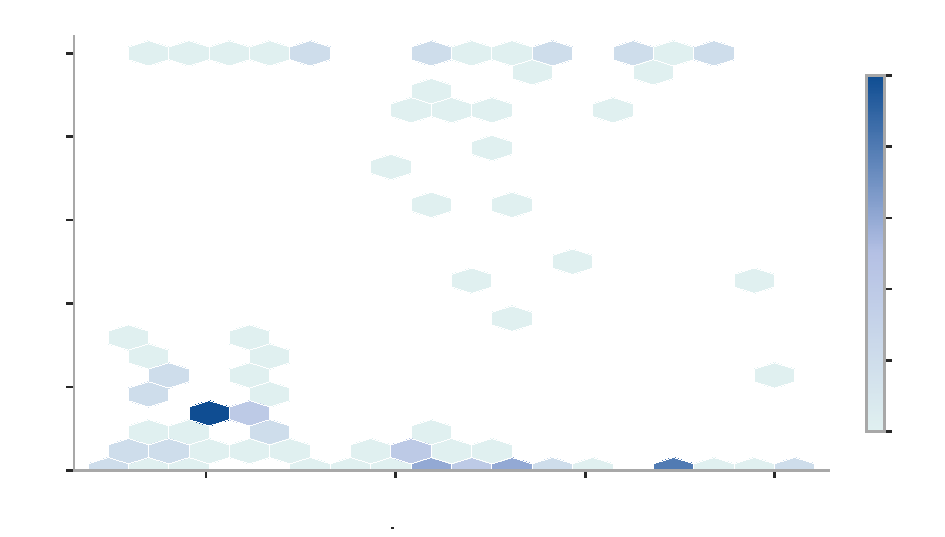
\includegraphics[width=160mm]{../求解/正式图件/q1-F01.pdf}
\caption{官方计算图结构分布}\label{fig:q1-f01}
\end{figure}

\begin{figure}[htbp]\centering
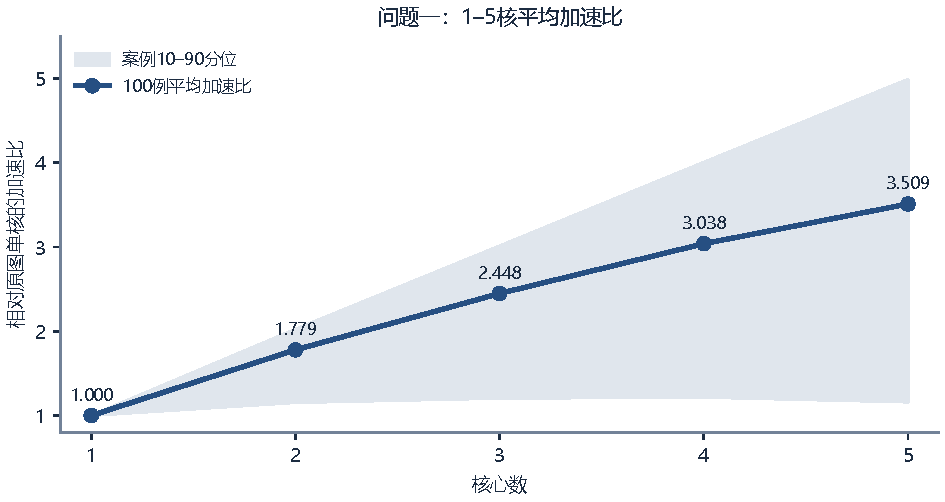
\includegraphics[width=160mm]{../求解/正式图件/q1-F02.pdf}
\caption{问题一核数扩展的平均加速比}\label{fig:q1-f02}
\end{figure}

各核数的平均加速比分别为$1.0000,1.7789,2.4477,3.0384,3.5093$。其增量递减，既反映并行工作被逐步分尽，也反映共享DDR、边界COPY与固定等待无法按核心数同比缩短。图~\ref{fig:q1-f03}把案例分层，使宽图与单块占优图的表现不被混为一种平均规律。逐例检查还发现26个算例在某一步增核后加速比下降，故不能把核数增加视作逐例单调改进；这些方案没有违反校验规则，而是完整事件模拟中的搬运、切换和调度次序共同变化。

\begin{figure}[htbp]\centering
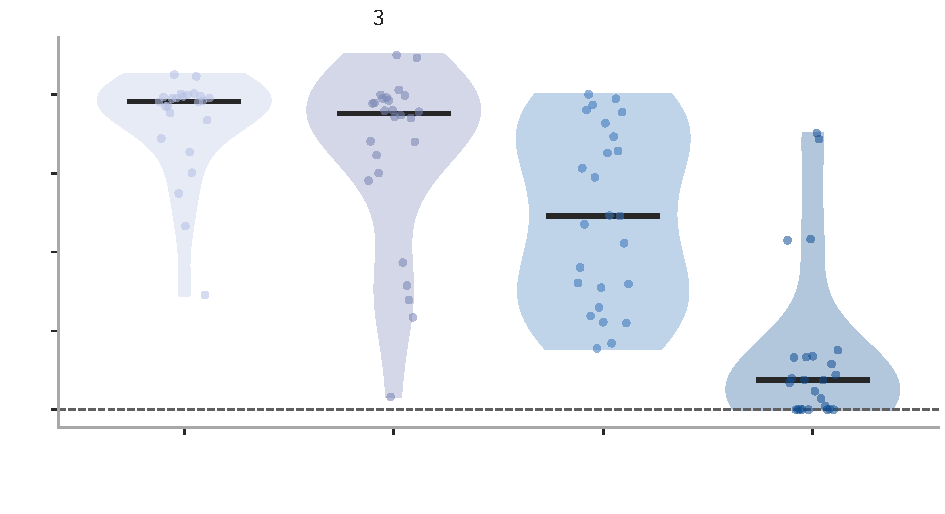
\includegraphics[width=160mm]{../求解/正式图件/q1-F03.pdf}
\caption{图结构分层与加速}\label{fig:q1-f03}
\end{figure}

五核最优候选的选择频数为连通块70例、深度分段22例、分批8例。连通块占多数，说明在这些输入中保持依赖块完整、减少跨子图搬运通常有利；但另30例需要对并行度或大Task求解成本作出折衷。图~\ref{fig:q1-f04}对照五核加速比与新增DDR搬运，并以操作数编码输入规模；零新增搬运落在轴原点。图~\ref{fig:q1-f05}将最大连通块大小和占比分箱，显示深度分段候选胜出的实际频率与每格样本数。两图共同约束“切得越细越好”的直觉：收益必须与新增传输和同步一起解释，不能把任一代理量当作官方目标。

\begin{figure}[htbp]\centering
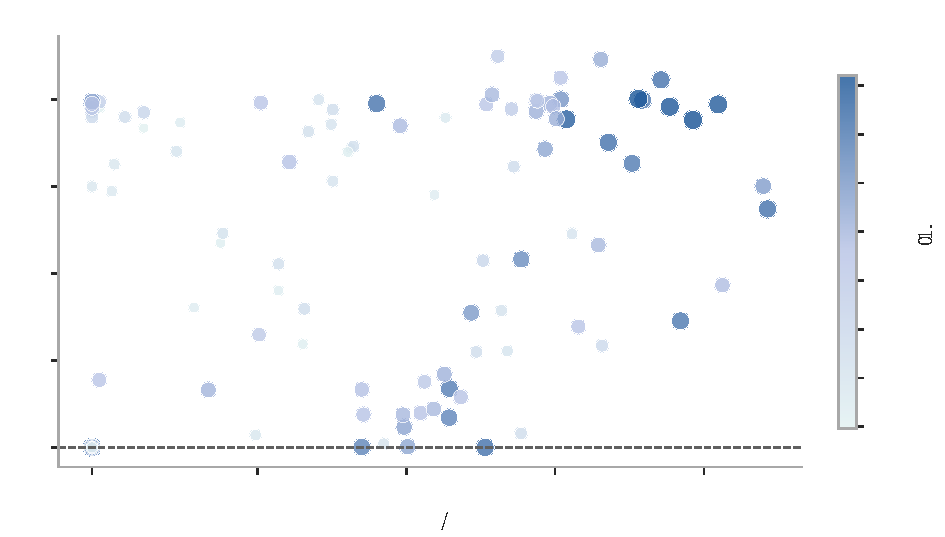
\includegraphics[width=160mm]{../求解/正式图件/q1-F04.pdf}
\caption{并行收益与新增搬运}\label{fig:q1-f04}
\end{figure}

\begin{figure}[htbp]\centering
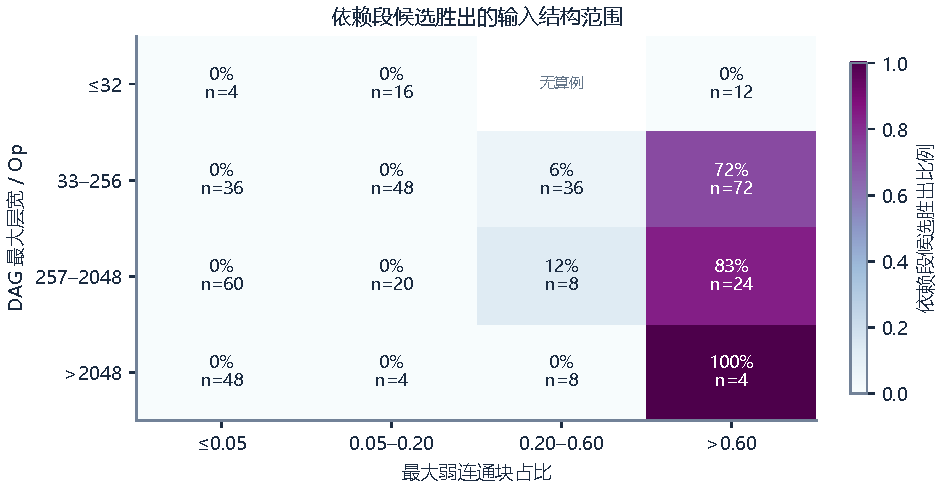
\includegraphics[width=160mm]{../求解/正式图件/q1-F05.pdf}
\caption{结构分箱中的候选胜率}\label{fig:q1-f05}
\end{figure}

最后，图~\ref{fig:q1-f06}报告候选评估的实际运行耗时与该候选相对同配置最佳完成时间的比。横轴是官方评估器处理候选的墙钟耗时，而不是所生成方案在处理器上的完成周期，也不含完整候选生成时间；因此只用来说明搜索预算与候选质量的折衷，不能作为题目加速比的分母。

\begin{figure}[htbp]\centering
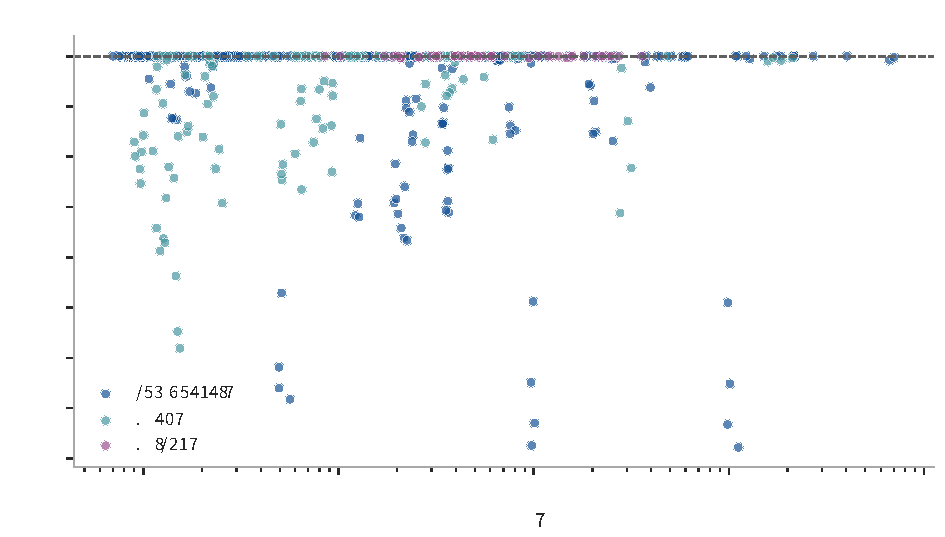
\includegraphics[width=160mm]{../求解/正式图件/q1-F06.pdf}
\caption{候选评估时间与规模}\label{fig:q1-f06}
\end{figure}

% Generated model comparison; edit scientific report and rerun the builder.
\noindent 本问是有显式约束和官方仿真目标的计算图组合优化；100 个图不提供最优方案标签，直接评价候选方案可复核，学习模型没有可验证的训练目标。\par


\subsection{结构分层的候选适配证据}

仅用总体五核均值无法检验候选构造是否符合图结构。为此令 $f$ 为最大弱连通块中的非 COPY 操作数占全部非 COPY 操作数的比例，按预先给定的四个范围对正式100例作互斥分层。表~\ref{tab:q1-structure-deep}从同一逐例记录重算各层的五核平均加速比、收缩 DAG 深度中位数与胜出候选频数；一个案例只计入一层。这里的深度是边数意义下的最长前驱层号，不是设备周期，不能直接与完成时间相减。四层样本量分别为38、21、13和28，因而表中的均值不是同样精度的总体估计，尤其不能把分层差异解释成随机试验中的处理效应。

\begin{table}[htbp]\centering
\caption{五核最大弱连通块占比分层的方案与收益}\label{tab:q1-structure-deep}
\small\begin{tabular}{lrrrrr}\toprule
最大块占比 $f$ & 算例数 & 平均加速比 & DAG深度中位数 & 连通块 & 分段/分批 \\ \midrule
$f\leq0.05$ & 38 & 4.6200 & 18.5 & 30 & 0/8 \\
$0.05<f\leq0.20$ & 21 & 3.8113 & 37.0 & 21 & 0/0 \\
$0.20<f\leq0.60$ & 13 & 3.6504 & 102.0 & 11 & 2/0 \\
$f>0.60$ & 28 & 1.7098 & 211.5 & 8 & 20/0 \\
\bottomrule\end{tabular}\end{table}
\begin{table}[htbp]\centering
\caption{问题一相邻核数下降的真实配置次数}\label{tab:q1-nonmonotone-deep}
\small\begin{tabular}{lrrr}\toprule
核数变化 & 加速比下降配置 & 同时换候选族 & 同时新增搬运增加 \\ \midrule
1→2 & 0 & 0 & 0 \\
2→3 & 7 & 0 & 7 \\
3→4 & 12 & 0 & 11 \\
4→5 & 22 & 1 & 19 \\
\bottomrule\end{tabular}\end{table}


最大块占比不超过$0.05$的38例，五核平均加速比为$4.6200$；其中30例由整块分配胜出，8例由分批候选胜出，深度中位数仅$18.5$。这组图的独立块多，分核时通常不必切断大型依赖块，所以低边界搬运与负载均衡可以同时实现。相反，在$f>0.60$的28例中，平均加速比为$1.7098$，深度中位数为$211.5$；20例需要深度分段，只有8例保持整块候选。该表给出构造策略与图结构相吻合的实测证据：块占比高时仅以整块为不可分单元，容易留下过大的串行片段。但分段胜出不等于高占比导致低收益的因果证明，因为最大块占比、DAG深度、操作周期、张量体积与带宽需求都随案例一起变化。

中间两个范围也有独立价值。$0.05<f\leq0.20$的21例全部选择连通块，均值$3.8113$；$0.20<f\leq0.60$的13例中只有2例改选分段，均值$3.6504$。这表明分段不是“块稍大便启用”的静态开关。其额外并行机会必须足以抵销 Task 等待和新增 DDR 搬运，最终仍以官方全局时间决定。表中把胜出频数与深度一起列出，也避免仅从图~\ref{fig:q1-f03}的分布形状推断具体哪个候选胜出。本文没有在分层后回改$2500$、$600$或$800$等构造阈值；这些数值固定于候选生成，分层表只是事后解释结果。

\subsection{结构代理量的反例检验}

分层均值显示趋势，但只有逐例反查才能判断最大块占比能否作为单独的决策规则。表~\ref{tab:q1-counterexamples}特意选取两例“小最大块但收益低”和两例“整图为单块但收益高”的正式五核结果。四例都来自原始100例，没有重新抽样或改变官方配置；其操作数、深度、最大层宽、搬运量和实际胜出候选均由同一逐例记录读取。这里的“收益低、高”是相对于同层总体趋势的描述，表中没有把案例从统计样本剔除。

\begin{table}[htbp]\centering
\caption{最大块占比不能单独预测五核收益的四例}\label{tab:q1-counterexamples}
\small\begin{tabular}{crrrrrc}\toprule
算例 & 最大块占比 & DAG深度 & 最大层宽 & 新增搬运/MiB & 加速比 & 胜出族 \\ \midrule
083 & 0.0323 & 125 & 31 & 14.36 & 2.3911 & 连通块 \\
092 & 0.0070 & 125 & 142 & 69.70 & 2.4555 & 分批 \\
062 & 1.0000 & 29 & 2181 & 22.83 & 4.5093 & 分段 \\
063 & 1.0000 & 27 & 817 & 8.57 & 4.4328 & 分段 \\
\bottomrule\end{tabular}\end{table}


算例083的最大块只占$0.0323$，却仅有$2.3911$倍五核加速；其DAG深度为125、最大层宽31，新增搬运约$14.36$ MiB。算例092的最大块占比更低，仅$0.0070$，但胜出的是分批候选，新增搬运约$69.70$ MiB，加速比$2.4555$。这两例说明“小块多”只表达可分配单元丰富，不说明张量边界便宜，也不说明所有可并行块会在资源争用下同时完成。尤其分批候选可能为降低超大Task的官方排布开销而被选中，其最终搬运代价必须一并报告。

反向的算例062与063最大块占比都是1，也即非COPY操作处于一个弱连通块，却分别达到$4.5093$和$4.4328$倍。两图的最大同层宽度分别为2181和817，远高于其深度29和27，深度分段能从同一个连接块中提出有用的并行片段。与算例016那种深度很长且宽度仅12的单块图相比，单块身份并不能确定可并行性。最大块占比衡量的是连通性，DAG深度和宽度衡量依赖方向上的并行机会，边界张量大小则决定让这些机会落在多核上要付出的传输成本。三个维度没有一个可以替代全局事件评估，但联合查看能解释为什么同一候选规则在不同图上产生不同效果。

这个反例检验也给下一轮候选设计指出具体方向：对占比高且宽度大的图，应尝试围绕依赖层内的可交换操作划分，同时限制边界张量总量；对占比低但COPY仍大的图，则应检查许多小块是否共享同一张量输入、是否被调度到过多不同核心。上述策略尚未成为本次正式结果，本文不把它们写成已验证算法或成绩。当前提交方案只使用前述三个已经逐例合法评估的候选族。

\subsection{合法性与离散事件目标的连接}

切图候选之所以可用于正式比较，首先依赖结构上的封闭性。令消去 COPY 端点后的非 COPY 依赖 DAG 为 $G'=(V',E')$，弱连通块集合为 $\mathcal C$。每个 $v\in V'$ 属于且仅属于一个弱连通块；若一条边 $(u,v)\in E'$ 的两个端点处于不同块，这两个块本应由该边连接，与弱连通定义矛盾。因此整块分核时，块间没有遗漏的原图依赖；同核多个块的固定排列只附加执行顺序，不会删除一条先后约束。每个操作恰好被指派一次，故块到核心、核心到子图的映射同时满足唯一覆盖和编号完备。

深度分段候选另令 $d(v)$ 为从任一源点到 $v$ 的最长依赖路径边数。对每条依赖边 $(u,v)$ 有 $d(v)\geq d(u)+1$。把有序深度轴切成相邻区段后，跨区段边只能由早段指向晚段；同一区段内再按弱连通块分割，区段内部不同块之间不存在依赖边。于是以“区段、核心”为子图并按区段序编号时，任何收缩后的边都不可能由晚段回到早段，也不可能形成区段内的块间环。该推导解释了候选构造的合法性来源，但不证明所选方案时间最短；具体容量约束和所有细节仍交给官方校验器与独立时间线检查。

全局 Makespan 是所有核心、Pipe 和共享资源上的事件最终完成时刻，可以写为 $T=\max_e t_e^{\mathrm{finish}}$。它一般不等于各核计算周期之和，也不等于简单的“最长链计算量加总搬运量”：COPY可能与计算重叠，多个核心的DDR请求又会竞争同一带宽池，固定 Task 等待也会改变后续事件次序。因此粗负载$w(C)$只在候选生成时平衡工作量，不作为正式目标的近似分数；深度$d(v)$只保证依赖方向，不代表纳入资源争用后的关键路径。本文的最终选择规则是在同一图、同一核数下对实际成功通过官方评估的候选取最小$T$，其保证仅相对于这组已评估候选成立。没有对所有合法切图与同核排序枚举，不能声称全局最优或给出未经证明的最优性缺口。

\subsection{增核非单调性与稳健性边界}

逐例核数曲线提供了均值曲线之外的反例。表~\ref{tab:q1-nonmonotone-deep}把四次相邻核数变化分别统计：从一核到两核没有下降配置；二到三、三到四、四到五核分别有7、12、22个下降配置。四列相加为41次“案例—核数转移”，涉及26个不同案例，不能把41误写成41个图。下降转移中仅1次同时更换了候选族，而37次伴随新增搬运量上升；后一个并发关系支持继续检查跨核张量，但不构成搬运单独造成下降的因果识别。同一候选族在两个核数下仍可能产生不同的块分配和Task顺序，故“候选族没变”也不是严格固定方案的反事实。

该现象决定了提交策略应保留每个要求核数的独立方案，而不是把五核的划分机械删核后视作二至四核答案。对图结构极宽的案例，额外核心可利用互不依赖的块；对长链或高边界流量案例，增加核心会使同步与COPY的相对成本上升。仅当候选在该核数经过合法性检查、官方全局评估并完成结果核验后，其时间才进入该核数的逐例成绩。表~\ref{tab:q1-nonmonotone-deep}同时限定了本文的稳健性主张：平均收益随核数增加，并不意味着100条个体曲线逐条单调；后续改进应把“新增核是否真正释放可并行依赖”纳入候选筛选，而不改变官方评价口径。

\subsection{结果核验与本问结论}

逐例结构诊断给出了均值无法表达的两端。算例016有$17995$个非COPY操作，全部属于同一弱连通块；其收缩DAG深度为$2441$、最大同层宽度仅$12$，五核候选仍选整块方案，完成周期$7715523$，相对原始单核的加速比恰为$1$。这个实例表明，核数可用并不意味着存在足够的独立块可直接分配。相反，算例059仅有$2752$个非COPY操作却分成$64$个弱连通块，最大块占比$0.015625$，五核整块分配后的完成周期为$150782$，加速比达到$5.5011$。它超过理想线性值$5$并非计时错误：本题基准是原始整图的官方单核时间，改变切图后也会改变核内排布及开销。因此不能把$k$误当成每个方案的严格加速上界。

两例都选连通块候选，但形成截然不同的响应，说明“胜出候选族”不足以描述方案质量。弱连通块数、关键路径深度和同层宽度必须与实际完成时间并读；即使图结构提示并行机会，也只能把它当作筛选候选的依据，不能跳过Task等待、COPY和共享带宽的官方评估。图~\ref{fig:q1-f03}的宽分布及图~\ref{fig:q1-f04}的成本散点正是对此逐例差异的总体检验。

每个最终方案均重新进行操作唯一覆盖、核心编号、无环和同核序列偏序核验，并保留官方原始响应与逐例方案。独立收集程序复算$T_1/T_k$、核对报告中的完成周期和新增搬运字段，再用事件时间线检查完成时刻；独立重算后，所选五百组方案的覆盖、时间线及官方响应交叉核验全部通过。此复核在官方评估器之外运行，避免把一次成功返回当成充分正确性证明。

本问方法保留三个有限、事先定义的候选族，没有枚举所有合法切图，故结果是可复核的可行调度而非全局最优性证明。尤其在大弱连通块内，深度分段最多八层，可能错过更细的依赖划分；而负载权重$w(C)$未显式预测共享带宽拥塞。图~\ref{fig:q1-f03}的低加速尾部提示后续应针对依赖关键路径和边界张量位置继续设计候选，但任何新策略仍需在同一官方评估链中成对比较。







\GMCMChapterEnd{4}
\section{问题二求解与分析}
\subsection{问题的描述与分析}

场景 B 将同一核心上的全部子图合并为一个 Task。这样，同核子图之间的中间张量可以保留在 L1 或 UB，跨核依赖才需要补入边界 COPY；代价是长期驻留的中间量可能占满私有缓存，迫使核内调度器进一步换入换出。问题一的划分不能直接凭 Task 数少就认定在新场景最优。图~\ref{fig:q2-overview} 对照同核复用、跨核通信以及完整时间线上的选择与验证。

% Generated figure only; description and reference belong before this input.
\begin{figure}[!htbp]
\centering
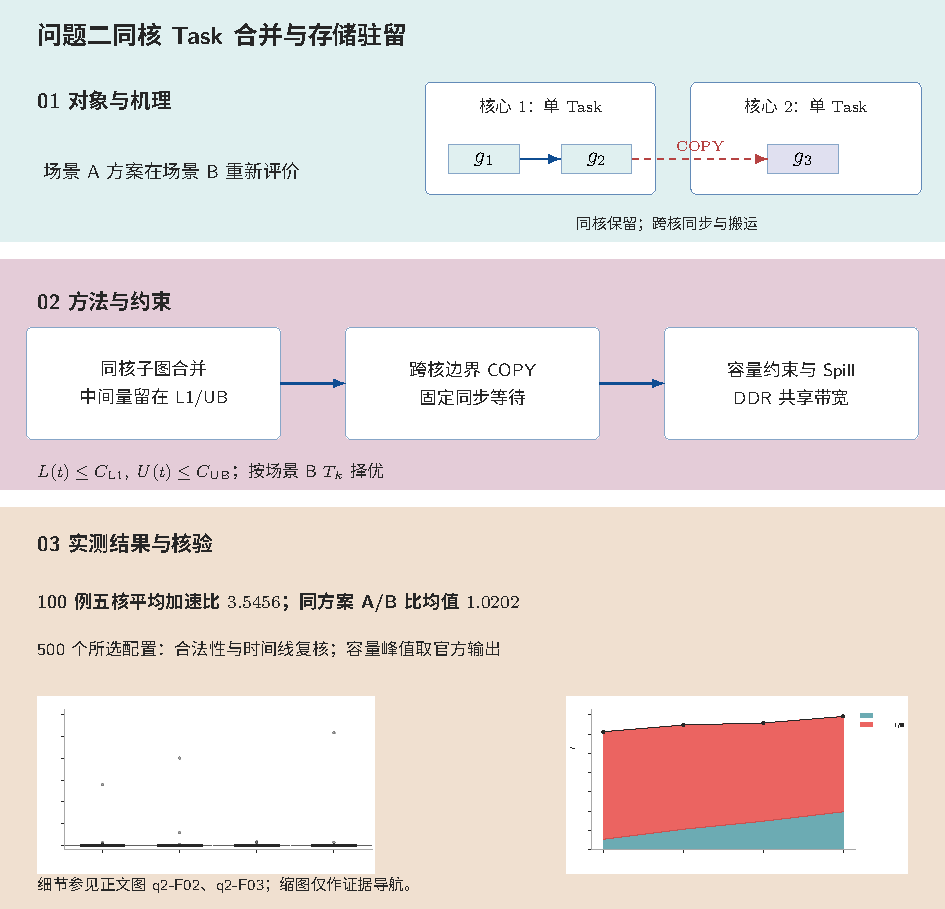
\includegraphics[width=160mm]{../求解/综合图/q2-overview.pdf}
\caption{问题二求解与核验总览}\label{fig:q2-overview}
\end{figure}
\FloatBarrier


图级算子融合可改变中间量的产生、驻留和搬运，TVM的端到端优化框架提供了类似的系统动机\cite{chen2018tvm}。本题场景B的合并对象和缓存语义由官方附件固定；我们仅在合法方案空间中比较它对全局时间线的影响。

\subsection{场景 B 的通信与存储约束}

仍采用问题一的 $g(i)$ 和 $a(g)$。若大小为 $s_j$ 的张量 $j$ 从源操作流向后继操作，且两端归属不同核心，场景 B 须在源核增加 COPY\_OUT、在目的核增加 COPY\_IN；接收端还要等待固定同步延迟。若两端在同一核心，即使所属子图不同，仍可在合并 Task 内保留核内数据，不因子图边界强制插入 DDR 搬运。这个规则与场景 A 的“每过子图边界都搬运”形成核心差别。

对每个时刻 $t$ 和每个核心，记 $L(t)$、$U(t)$ 分别为驻留于 L1 与 UB 的张量字节总量，需满足
\begin{equation}\label{eq:q2-capacity}
L(t)\le C_{\mathrm{L1}},\qquad U(t)\le C_{\mathrm{UB}}.
\end{equation}
其中 L1 容量 $C_{\mathrm{L1}}$ 与 UB 容量 $C_{\mathrm{UB}}$ 都来自题定固定配置。完整 Task 内部的拓扑顺序及必要 Spill 由题定核内调度器确定，所以本式并不等同于只在子图交界检查容量。若合并造成更高的驻留压力，评估器会插入换出与换入；新增 DDR 搬运由原图 COPY、分核边界 COPY 和 Spill 分解核对。

跨核依赖的延迟、共享 DDR 总带宽 $B_{\mathrm{DDR}}$ 及计算 Pipe 占用均按官方多核事件模拟器结算。其输入除了图和配置，只有两个方案字段：操作到子图的映射及各核心子图序列。我们不额外假定跨核 COPY 可以与特定操作完全重叠，也不以缓存可复用等同于缓存必然命中。

\subsection{切图复用与候选比较}

问题二继续采用连通块负载均衡、依赖深度分段以及宽图分批三个候选族，但在场景 B 下分别重评并重新排序。同核分批子图最终合入单个 Task，因此它的额外子图编号不必然造成场景 A 式清空；但分批次序仍可能改变核内拓扑排布和张量存活区间。深度分段虽然切出更多子图，也可能把共享输入关联的操作拉到同核，降低跨核边界；反之，若过多前驱被放到另一核心，则额外 COPY 与同步等待会抵消负载均衡收益。

采用场景B重新择优，对固定核数与算例，按官方场景 B 全局 $T_k$ 选择候选，完成时间并列时比较 $D_k$。为区分硬件规则收益与方案重新选择的收益，另把问题一的选中方案直接放到场景 B 评估，形成同一方案的 A/B 成对时长；场景 B 最优候选相对此固定方案的改善单独报告。两个比较不能混为一个“通信机制增益”。

\subsection{官方算例结果与分析}

场景B的正式结果同样覆盖100例、1至5核及三个预设候选族。图~\ref{fig:q2-f06}按题目要求给出逐例计算后汇总的1至5核平均加速比折线，单核基准与问题一相同。五核平均加速比为3.5456（无量纲），中位数$4.1473$，第10与第90百分位为$1.4066$、$4.9864$。图~\ref{fig:q2-f01}直接给出同一方案从场景A切换到B的逐例时长比，并按核数分层；比值小于1的点表明新场景也可能变慢，不能把均值正向差异解释为每例都获益。场景B五核候选频数为连通块67、深度分段25、分批8；相对场景A有少数算例发生候选切换。

\begin{figure}[htbp]\centering
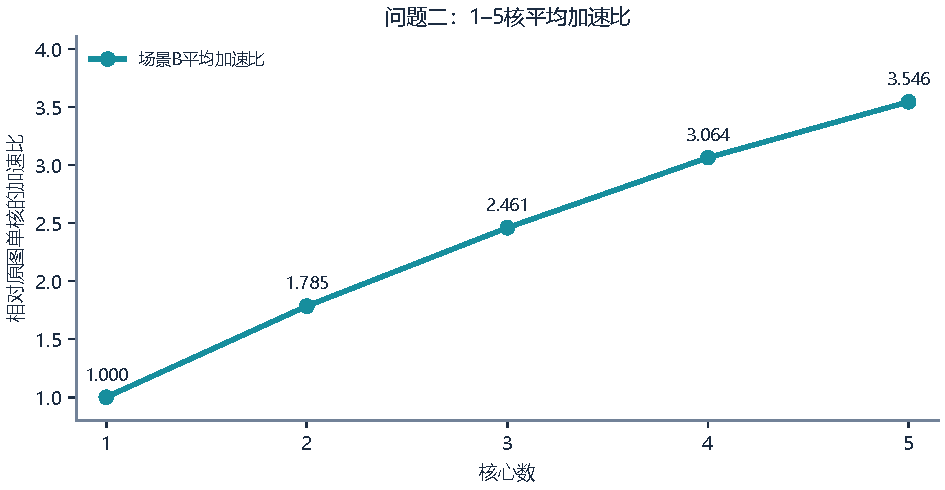
\includegraphics[width=160mm]{../求解/正式图件/q2-F06.pdf}
\caption{问题二核数扩展的平均加速比}\label{fig:q2-f06}
\end{figure}

对应的平均加速比依次为$1.0000,1.7850,2.4605,3.0644,3.5456$。从二核到五核仍持续增长，但相邻核数的绝对增量并不恒定；这些数是100个算例分别求比后的均值，不能把平均完成周期相除来替代。与图~\ref{fig:q1-f02}比较时，两图共用单核基准，因而差别来自场景规则和候选重选的共同作用。后面的同方案对照才将两者拆开。

\begin{figure}[htbp]\centering
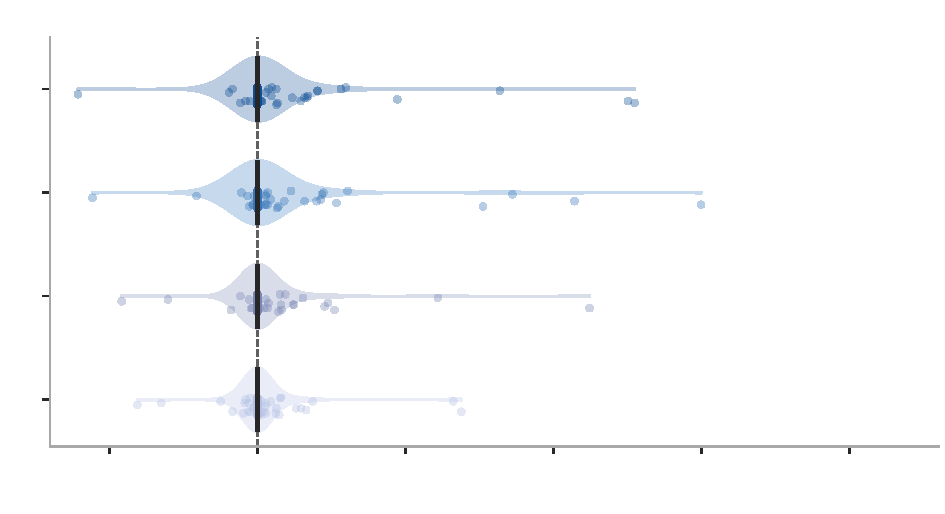
\includegraphics[width=160mm]{../求解/正式图件/q2-F01.pdf}
\caption{同方案场景收益分布}\label{fig:q2-f01}
\end{figure}

为了隔离机制，把问题一选中方案原样放入场景B。五核同方案时长比$T_A/T_B$的均值为$1.0202$，中位数为$1$，最小值$0.7577$，最大值$1.5096$。也就是说，Task合并并不保证逐例加速：个别算例因存储驻留和Spill反而变慢。另以问题二所选候选对同一场景B下的问题一候选作比较，平均再改善$1.0054$倍，中位数仍为$1$。图~\ref{fig:q2-f02}把硬件场景变化和重新择优分开呈现，避免将两种收益叠加成一个笼统结论。

\begin{figure}[htbp]\centering
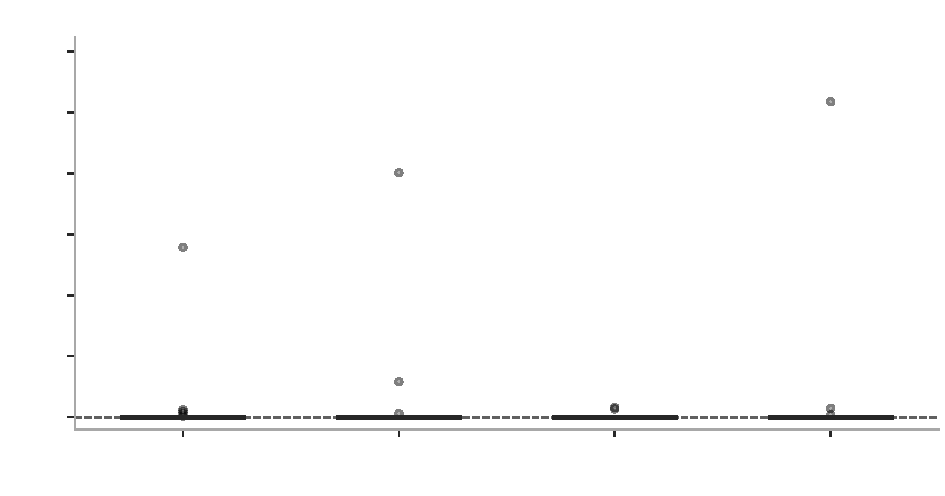
\includegraphics[width=160mm]{../求解/正式图件/q2-F02.pdf}
\caption{场景变化与方案重选}\label{fig:q2-f02}
\end{figure}

图~\ref{fig:q2-f03}按核数分解平均新增DDR搬运，区分切图边界和容量Spill。搬运总量与完成时间并不一一对应：同步等待、共享带宽争用、与计算Pipe的重叠都由事件模拟决定。因此这张图说明成本来源，最终择优仍使用官方全局Makespan。

\begin{figure}[htbp]\centering
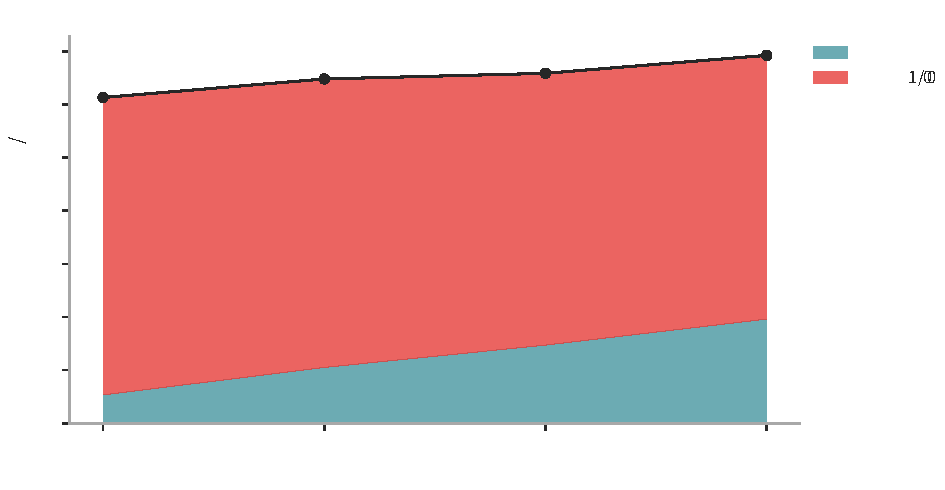
\includegraphics[width=160mm]{../求解/正式图件/q2-F03.pdf}
\caption{新增搬运来源分解}\label{fig:q2-f03}
\end{figure}

问题二的存储约束是逐时刻约束。图~\ref{fig:q2-f04}读取官方详细输出中的五核私有存储最大峰值，除以相应额定容量后同五核加速比对照。该图检视容量压力与调度收益的异质关系；峰值未超过容量只能证明已生成时间线的可行性，不能证明其他未搜索切图也满足约束。图~\ref{fig:q2-f05}则在每个算例的五核成对点上同时表示加速比变化与新增搬运变化；一部分点在“加速且减搬运”象限，但也能看到代价与性能方向不一致的案例，说明不能以搬运字节独立替代完成周期。

\begin{figure}[htbp]\centering
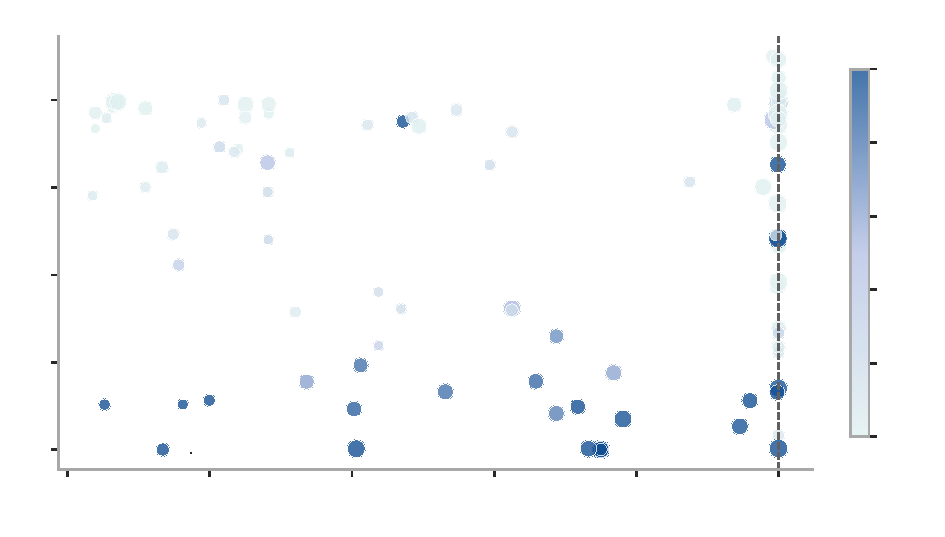
\includegraphics[width=160mm]{../求解/正式图件/q2-F04.pdf}
\caption{容量压力与调度收益}\label{fig:q2-f04}
\end{figure}

\begin{figure}[htbp]\centering
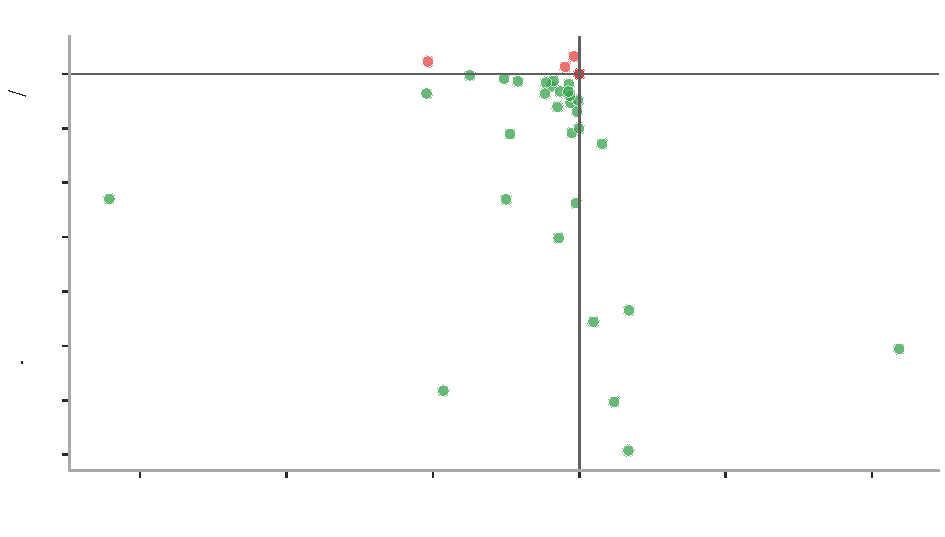
\includegraphics[width=160mm]{../求解/正式图件/q2-F05.pdf}
\caption{加速与搬运的成对变化}\label{fig:q2-f05}
\end{figure}

表~\ref{tab:q2-paired-cases}从两端算例核查两种收益的分离。算例062的两问五核候选都为深度分段，因而$633094/835503=0.7577$直接是同一方案切换场景的比值；场景B虽然比A少了新增DDR搬运，完成周期却增加，说明传输字节下降并不足以保证全局时间缩短。算例071则恰好相反：固定问题一的连通块方案在场景B中仍用$18919$周期，规则本身没有带来时长收益；问题二改选深度分段后才缩至$12470$周期。若只看最后的$1.5172$倍改善，就会把方案适配误写成Task合并本身的效果。

\begin{table}[htbp]\centering
\caption{五核两端算例的同方案与重选对照}\label{tab:q2-paired-cases}
\small
\begin{tabular}{c c r r r r}
\toprule
算例 & 问题一候选 & $T_A$ & $T_B$同方案 & $T_B$重选 & 同方案$T_A/T_B$ \\
\midrule
062 & 深度分段 & 633094 & 835503 & 835503 & 0.7577 \\
071 & 连通块 & 18919 & 18919 & 12470 & 1.0000 \\
\bottomrule
\end{tabular}
\end{table}

上述算例的每个完成周期都来自同一官方事件模拟口径，表中没有用局部Task时间拼接全局Makespan。算例062的逆向差异提示继续检查私有存储驻留、Spill和同步时间；然而现有输出只能证明这些机制共同参与，不能仅凭搬运总量断言某个单项是唯一原因。算例071的重选收益说明场景B下子图划分仍然是决策变量，尽管同核子图最后合入一个Task。

% Generated model comparison; edit scientific report and rerun the builder.
\noindent 本问是有显式约束和官方仿真目标的计算图组合优化；100 个图不提供最优方案标签，直接评价候选方案可复核，学习模型没有可验证的训练目标。\par


\subsection{规则改变与候选重选的逐核分解}

问题二同时更改执行语义与可采用的切图方案，若直接比较问题一、二各自的最优成绩，就无法知道改善来自哪里。对同一算例和核数，记问题一所选方案为$p_A$，问题二所选方案为$p_B$。本文实际保存三次可比评价：场景A的$T_A(p_A)$、场景B但固定方案的$T_B(p_A)$，以及场景B重选后的$T_B(p_B)$。逐例有精确恒等式
\begin{equation}\label{eq:q2-decompose}
\frac{T_A(p_A)}{T_B(p_B)}=
\underbrace{\frac{T_A(p_A)}{T_B(p_A)}}_{\text{规则效应（同方案）}}
\underbrace{\frac{T_B(p_A)}{T_B(p_B)}}_{\text{重选效应（同场景）}}.
\end{equation}
它只是同一实例中三个实测时间的代数分解，并未假设两种效应独立。汇总100例时必须先逐例计算比值再求均值；一般来说，两个逐例因子的均值之积不等于总比值的均值，更不能把三问各自报告的平均加速比直接相除当作式~\eqref{eq:q2-decompose}的第一项。

表~\ref{tab:q2-paired-deep}把二至五核逐级列出。表中“改善/变差”只比较同一方案下的场景A与B，“重选受益”只比较两个场景B方案；等于1的案例不计入任一方向。二核有21例在规则改变后改善、13例变差，五核为24例改善、6例变差，仍有70例无时长变化。五核规则效应的逐例平均为$1.0202$，但其最小值在算例062只有$0.7577$，所以“合并Task平均有益”不能改写成“合并Task对每张图有益”。二至五核的重选受益例数仅5、3、2、3，均值接近1；这是当前三个有限候选族之间的观察，既不说明场景B无需优化，也不表示所有合法划分已被比较。

\begin{table}[htbp]\centering
\caption{场景B逐核成对比较与搬运来源}\label{tab:q2-paired-deep}
\small\begin{tabular}{rrrrrrr}\toprule
核数 & 同方案均值 & 改善/变差例数 & 重选均值 & 重选受益例数 & 候选切换 & Spill例数 \\ \midrule
2 & 1.0053 & 21/13 & 1.0031 & 5 & 7 & 44 \\
3 & 1.0097 & 20/7 & 1.0046 & 3 & 5 & 40 \\
4 & 1.0217 & 23/8 & 1.0003 & 2 & 2 & 37 \\
5 & 1.0202 & 24/6 & 1.0054 & 3 & 3 & 37 \\
\bottomrule\end{tabular}\end{table}


候选族切换次数与重选严格受益次数不同，也值得分开读。二至五核分别有7、5、2、3个案例改变了胜出候选族，超过同核数严格时长改善的5、3、2、3例，说明某些不同族候选在官方全局时长上并列，需靠次级搬运量或固定平局规则确定最终方案。即使候选族不变，具体核心指派也可能变；表中的“切换”只统计族名，不能充当逐字节的方案身份校验。另一方面，五核算例002在固定深度分段方案时由场景A的$83172$周期降到场景B的$55096$周期，比值$1.5096$，而重选因子恰为1。这与前述算例071构成相反的机制示例：002主要见到规则变化的实测收益，071的$1.5172$倍则主要来自场景B重新选出分段方案。两例共同说明必须保留式~\eqref{eq:q2-decompose}的中间评价。

\subsection{边界搬运、Spill与驻留约束}

场景B省去同核子图之间的重复外存往返，但不会让跨核边界和私有存储容量消失。把一个跨核张量的发送端、接收端视为有序依赖，只有两端核心不同才需要跨核边界COPY；这可以用指示量 $I_{uv}=\mathbf 1\{a(g(u))\ne a(g(v))\}$ 标记。张量边的大小与$I_{uv}$乘积有助于候选构造时识别潜在边界流量，但不等于最终的官方新增搬运总量：原始COPY、张量复用次数、Spill以及评估器的具体图转换规则都要计入。本文因此仅以该量作代理，不拿它替换真实 $D_k$，结果图~\ref{fig:q2-f03}用官方详细响应把边界COPY和Spill分开。

核内驻留同样是时间相关约束。若 $\mathcal L_k(t)$ 和 $\mathcal U_k(t)$ 分别表示核心$k$在事件时刻$t$仍位于L1和UB的张量集合，合法峰值要求 $\sum_{j\in\mathcal L_k(t)}s_j\leq C_{\rm L1}$ 与 $\sum_{j\in\mathcal U_k(t)}s_j\leq C_{\rm UB}$ 在全部实际时刻成立。不能把一个Task里出现过的所有张量静态相加当作峰值，也不能用平均占用率取代峰值。合并Task使同核边界数据可能延长驻留时间；即使跨核COPY字节下降，私有缓存更早溢出也可能出现Spill，进而改变DDR请求排队与计算Pipe的空闲区间。本文用官方输出中的逐核峰值与Spill字节核验这一点，没有另造一个与官方事件顺序不一致的内存模拟器。

五核正式所选方案的100例汇总中，新增边界搬运约$392.3$ MiB，Spill约$992.1$ MiB；按这两项总量计算，Spill占新增搬运约$71.7\%$。这是字节量的跨案例求和，不是“71.7\%的案例发生Spill”：五核实际有37例Spill大于零。两个统计口径不同，正说明少数较重的存储压力图可主导总字节数。二至五核发生Spill的例数为44、40、37、37；随核数增加这个计数略降，而边界搬运总量上升，不能据此推出某一种机制单独决定完工时间。图~\ref{fig:q2-f04}的容量峰值与收益散点以及图~\ref{fig:q2-f05}的速度—搬运双轴，分别用于检验上述容量与时间响应是否一致。

\subsection{候选族内的存储代价交叉核查}

总字节均值还有一个隐患：不同类型的图规模和结构混在一起。表~\ref{tab:q2-family-crosscheck}按五核问题二最终胜出的候选族重新分组，分别计算官方详细输出中的边界搬运和Spill平均量，并给出相应案例的平均加速比。这是事后条件描述，不能被解释为把同一批图随机分配到三种算法后的处理效应；尤其某一族只会在它相对有利的图上成为胜者。分组表的意义是核对“哪类已选方案携带怎样的实际资源账”，而不是据均值挑一个永远最优的算法。

\begin{table}[htbp]\centering
\caption{五核胜出候选族的搬运组成与收益}\label{tab:q2-family-crosscheck}
\small\begin{tabular}{lrrrrr}\toprule
候选族 & 例数 & 边界搬运均值/MiB & Spill均值/MiB & Spill例数 & 平均加速比 \\ \midrule
连通块 & 67 & 2.98 & 6.59 & 22 & 3.9476 \\
深度分段 & 25 & 2.69 & 4.15 & 8 & 2.1728 \\
分批 & 8 & 15.68 & 55.85 & 7 & 4.4693 \\
\bottomrule\end{tabular}\end{table}


连通块族在67例中胜出，其边界搬运均值$2.98$ MiB，Spill均值$6.59$ MiB，22例Spill大于零，平均加速比$3.9476$。深度分段族对应25例，边界均值$2.69$ MiB、Spill均值$4.15$ MiB，平均加速比却仅$2.1728$。不能据此称分段“比整块慢”，因为分段主要被难以整块并行的高连通图选中，所面对的图结构不同。分批族只有8例，平均加速比$4.4693$，但边界和Spill均值高达$15.68$与$55.85$ MiB，7例发生Spill。这些案例能凭自身图宽与短任务取得明显并行收益，同时承担很高的绝对搬运成本；高收益与高搬运在不同图规模下完全可以共存。

分组结果还解释了为何只在同一图、同一核数下比较候选，不能把表内三个族的平均加速比直接排序作为部署规则。严格的候选比较需要固定图、硬件参数和核数，然后把每个合法候选交给同一官方评估链。表~\ref{tab:q2-family-crosscheck}没有替代这一步，而是对最终选择作资源诊断。若后续要检验“分段是否降低Spill”这类因果命题，需在同一批案例上保留所有候选的Spill、峰值与时间，并显式处理不合法或超时候选；目前的胜出族条件均值尚不足以给出该结论。

官方详细响应、所选方案和独立核验记录的关联也遵循这个单位：同一案例的二至五核四个方案各自保存，不借用其它核数的时间线。核验程序首先检查非COPY操作覆盖与编号、收缩图无环和同核次序，再比对官方给出的全局完成周期、峰值与新增搬运拆分。出现候选评估失败时，不把缺失时间记为零或无穷大后参与均值；选中方案必须有可读取的官方成功响应。本次500个所选配置全部通过逐项交叉核验，这一通过数反映的是结果可复查性，不是未选候选的全局最优性证明。

\subsection{可迁移结论的范围}

这些逐核比较只针对题目给出的100张图、固定硬件配置和当前候选集合。对同核边界密集且仍有存储余量的图，合并Task可能减少DDR往返；对长寿命张量多、原已逼近L1或UB容量的图，同一改变也可能增大Spill。这个判断是从已观测的成对结果、搬运分解及题定机制提出的条件性解释，不是对任意NPU的性能保证。若移到另一处理器，必须先重测固定等待、私有容量、COPY转换与带宽争用，之后再比较$T_A(p_A)$、$T_B(p_A)$和$T_B(p_B)$；单纯复用本文的胜出频数不能代表新设备的最优策略。当前研究在五核处仍有部分案例由分段候选胜出，表明跨核边界的位置与同核驻留应在后续候选中联合优化，而不是只减少一种COPY数量。

\subsection{容量与时间线核验}

独立核验重新读取官方输出中的操作时间线，确认所选方案的合法性与完成周期一致。张量驻留峰值和COPY分解取自官方详细输出；其中L1、UB峰值均在题定容量内，本文没有对这两个峰值另写独立内存模拟器。独立重算后，所选五百组方案的覆盖、时间线及官方响应交叉核验全部通过。逐例增核并非单调：场景B有24个算例在至少一次增核时加速比下降，与固定同步及内存压力的解释相符，但不能仅凭该计数把原因归结为某一种COPY。

成对比较仍有两项边界：第一，所比的场景均由官方模拟器定义，未测真实硬件上的温度、功耗或抢占；第二，当前候选未针对UB/L1驻留区间显式优化，因此在Spill较重的图上可能还有改善空间。

对式~\eqref{eq:q2-decompose}的逐核结果还应检查“没有变化”的案例。二核固定方案切换场景后，21例严格变快、13例严格变慢，其余66例完成周期相等；五核相应为24例、6例和70例。均值略大于1并不表示大多数图都变快，而是少数受影响案例的幅度足以改变平均值。相等只说明官方全局Makespan未变，不能证明Task边界、COPY数量或私有驻留轨迹也完全相同：这些局部变化可能发生在非关键路径上。因此，评价场景B时同时保留逐例方向、完成周期和搬运拆分，比只报告一个平均倍数更能识别适用范围。

资源账也显示核数增加后的两种压力方向并不一致。按官方详细响应跨100例求和，二核所选方案的新增边界搬运约$106.8$~MiB、Spill约$1119.1$~MiB；五核分别约$392.3$~MiB和$992.1$~MiB。跨核边界总量增加，而Spill总量下降；这不能简化为“增核节省存储”或“增核只增加通信”。两组总量比较使用了不同核数下各自重新选出的方案，且聚合字节无法表示关键路径等待，故只能作为资源诊断。若要在新设备上预先约束最坏延迟或DDR预算，还须以逐图成对评估重新估计尾部风险，不能按本题总体均值直接指定核数。







\GMCMChapterEnd{5}
\section{问题三求解与分析}
\subsection{问题的描述与分析}

问题三保持场景 B 的 Task 与跨核同步结构，在 COPY\_IN 读共享输入时增加只读 L2 查询。Cache 命中走与 DDR 分离的读带宽池，未命中仍占用共享 DDR。FIFO 淘汰与容量决定后续复用能否发生；Cache 的时延收益不是命中次数的简单线性函数，因为并行 COPY 之间还会争用各自带宽。图~\ref{fig:q3-overview} 将共享读、FIFO 状态和同方案反事实比较连接到最终 Makespan。

% Generated figure only; description and reference belong before this input.
\begin{figure}[!htbp]
\centering
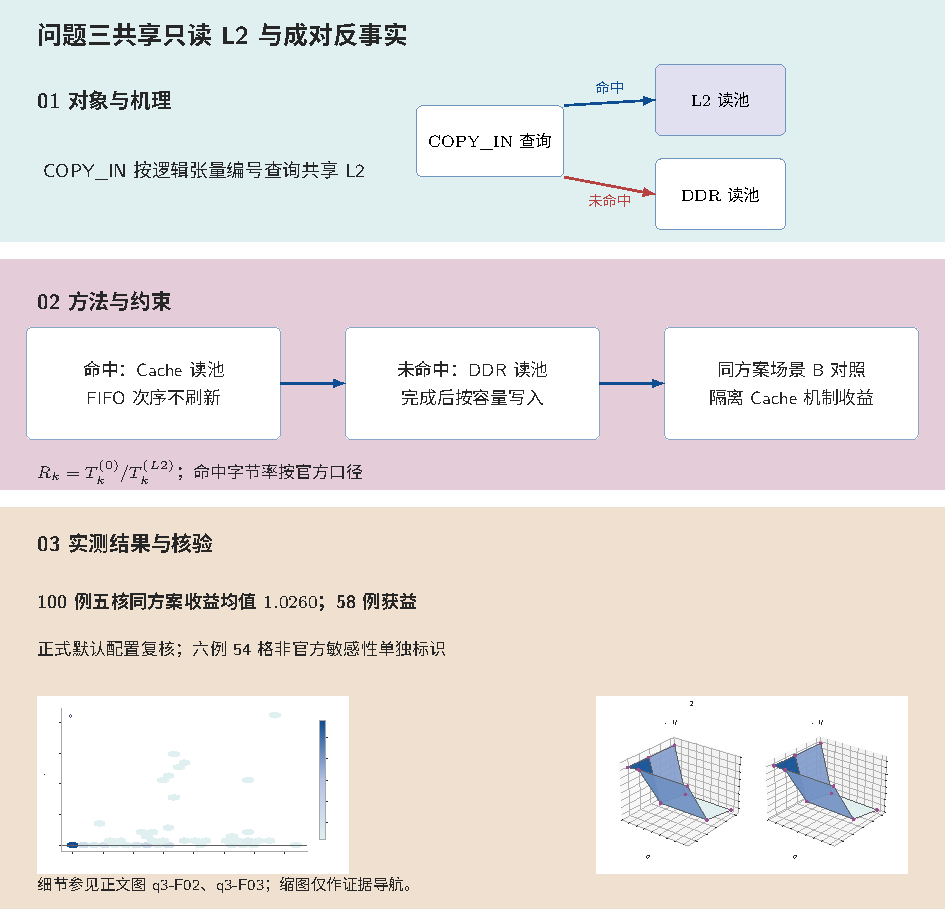
\includegraphics[width=160mm]{../求解/综合图/q3-overview.pdf}
\caption{问题三求解与核验总览}\label{fig:q3-overview}
\end{figure}
\FloatBarrier


存储层级的经典评价工作通过访问轨迹比较容量与替换策略下的命中行为\cite{mattson1970}。这启发本文同时报告L2命中字节和完成周期；然而题目使用不刷新次序的FIFO及两条独立读带宽池，不能直接把通用命中率公式套作本题的时延模型。

\subsection{只读 Cache 与成对评价模型}

对一次 COPY\_IN，先按张量逻辑编号查找 L2。命中时把所需字节交由 Cache 读带宽池，且不刷新该项 FIFO 顺序；未命中时从 DDR 读取，完成后按容量规则写入，只读 L2 不服务 COPY\_OUT。容量 $C_{\mathrm{L2}}$ 与读带宽 $B_{\mathrm{L2}}$ 由题定固定配置提供；单张量若大于容量就不缓存。DDR 的读写仍共享原带宽池，两个带宽池互相独立。

令同一图、同一核数和同一方案下，无 L2 与有 L2 的全局 Makespan 分别为 $T_k^{(0)}$ 与 $T_k^{(L2)}$。问题要求的 Cache 加速比是
\begin{equation}\label{eq:q3-cache-gain}
R_k=\frac{T_k^{(0)}}{T_k^{(L2)}}.
\end{equation}
另按官方口径，命中字节率为
\begin{equation}\label{eq:q3-hit-rate}
H_k=\frac{\text{L2命中 COPY\_IN 的字节数}}{\text{可查询 L2 的 COPY\_IN 总字节数}}.
\end{equation}
分母为零时按评估器的定义记录，不自行补造命中率。Cache 改变 COPY 完成顺序和全局争用，故 $R_k$ 未必与 $H_k$ 单调对应；结论依实际场景输出判断。

\subsection{方案适配与参数响应实验}

在固定官方配置下，对前两问的三个候选族重新用问题三评估器排序。选中方案之后，用完全相同的图和方案调用无 L2 的场景 B 评估器，再计算式~\eqref{eq:q3-cache-gain}，这样候选策略变化不会混入 Cache 收益。问题一、二、三各自可以选不同候选；若最终选中相同方案，仅说明该图上实测排序一致，不能推导一般情形必然相同。

容量与带宽的影响另做非官方参数敏感性实验：从正式 5 核案例按固定排序规则抽取不同 Cache 收益层的代表图，在工作区复制原配置后只改 L2 容量和读带宽。逐格对可用候选方案调用未改动的问题三评估器，记录固定默认方案的响应与该格重新择优的响应，并对比候选切换。它回答机制与方案适配方向；改动的配置不得并入题目要求的 100 例正式成绩，也不能用少量目的抽样推断 100 例平均收益。

\subsection{官方算例结果与分析}

在题定默认L2配置下，100例正式结果覆盖1至5核。五核平均加速比3.6104（无量纲），中位数$4.2231$，第10与第90百分位为$1.4609$、$5.0048$。其单核平均加速比为$1.0086$，可以高于1，因为分母仍是原始图的无L2单核基准。图~\ref{fig:q3-f06}按题目要求比较固定同一方案时无L2与有L2的1至5核平均加速比，两个序列都除以各算例原图无L2单核时间。图~\ref{fig:q3-f01}给出五种核数下同方案Cache收益比的经验累积分布；曲线在1附近快速上升，说明多数算例增益较小，而少数算例形成右尾。

\begin{figure}[htbp]\centering
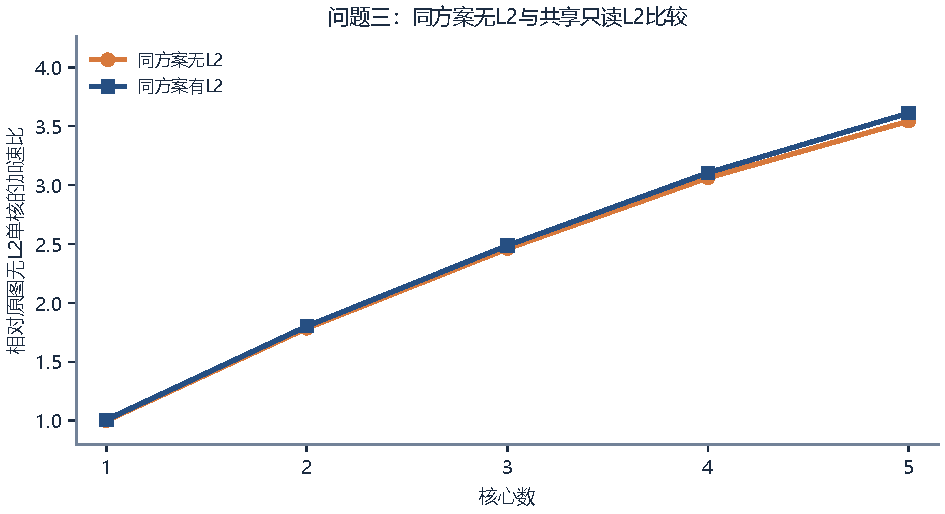
\includegraphics[width=160mm]{../求解/正式图件/q3-F06.pdf}
\caption{同方案无L2与有L2的核数比较}\label{fig:q3-f06}
\end{figure}

无L2与有L2曲线在核数1至5处的平均值分别为
\begin{align*}
(\bar S_k^{(0)})_{k=1}^{5}&=(1.0000,\ 1.7850,\ 2.4605,\ 3.0613,\ 3.5421),\\
(\bar S_k^{(L2)})_{k=1}^{5}&=(1.0086,\ 1.8026,\ 2.4873,\ 3.1044,\ 3.6104).
\end{align*}
两条线每个横坐标都使用相同算例与相同问题三选中方案；因此其垂直差异与方案重选无关。无L2曲线与问题二图~\ref{fig:q2-f06}接近但不完全重合，是因为问题二在无L2规则下选候选，而这里为隔离缓存机制固定问题三方案。这个细微差别也说明跨问题直接比较均值不足以识别单一硬件效应。

\begin{figure}[htbp]\centering
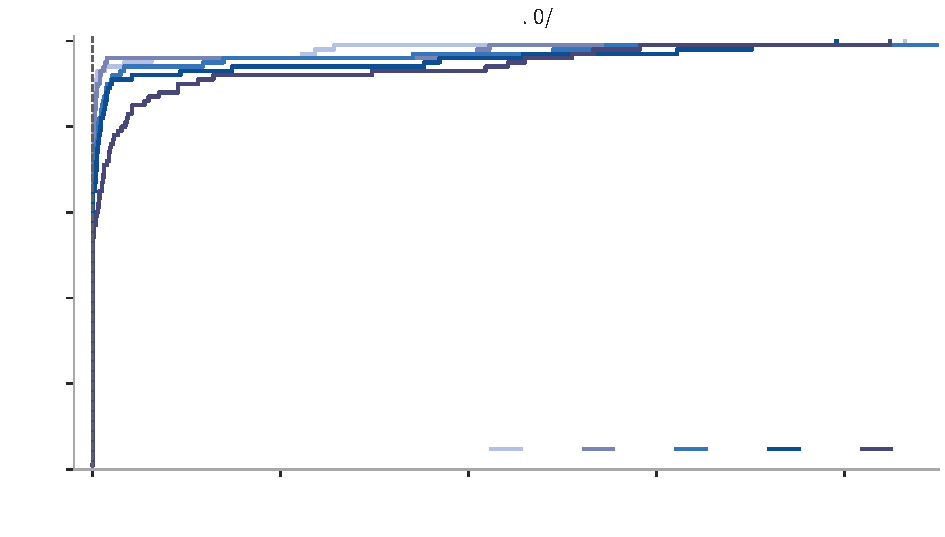
\includegraphics[width=160mm]{../求解/正式图件/q3-F01.pdf}
\caption{同方案Cache收益累积概率}\label{fig:q3-f01}
\end{figure}

五核同方案Cache比$R_5$均值为1.0260（无量纲），中位数$1.0001$，第90百分位$1.0464$；有正向收益的算例过半（58例）。平均逐例命中字节率为$21.29\%$，中位数$21.19\%$。最低$R_5$略小于1，表明FIFO与两个带宽池改变事件次序后，极小的逆向变化在官方模拟输出中确实可能发生。图~\ref{fig:q3-f02}把逐例命中字节率和同方案收益相对照。离散点与高密度区说明“命中率高”不是“完成时间按比例下降”的充分条件；还需看COPY是否落在关键路径，以及DDR/Cache带宽竞争与计算Pipe的重叠。

\begin{figure}[htbp]\centering
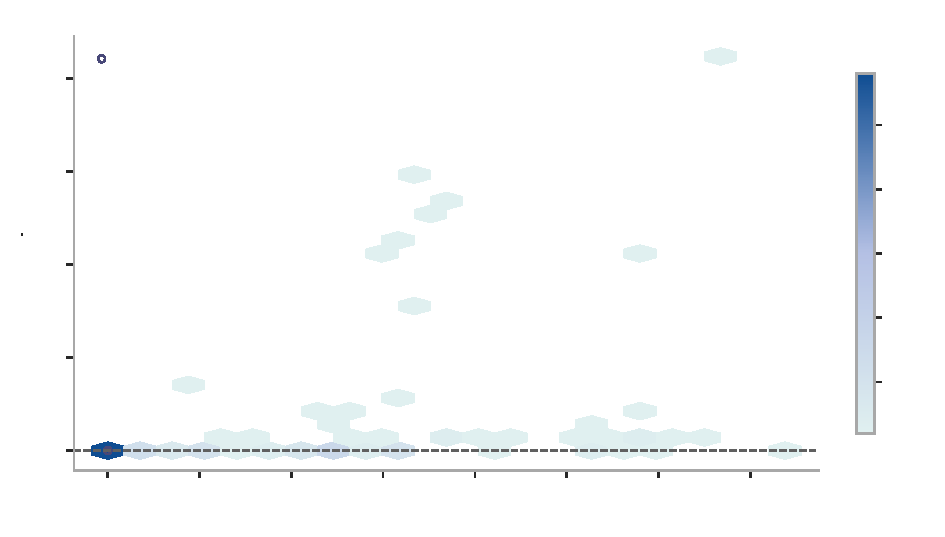
\includegraphics[width=160mm]{../求解/正式图件/q3-F02.pdf}
\caption{L2命中率与同方案收益}\label{fig:q3-f02}
\end{figure}

表~\ref{tab:q3-cache-cases}给出命中率与完成周期不能互相替代的逐例证据。算例083在固定的五核方案下，无L2与有L2分别需$442480$和$310731$周期，命中字节率$67.57\%$，收益比为$1.4240$。这证明在该案例的题定事件模型中，共享读开启后全局完工时间确实下降；汇总量本身还不能定位具体受益的关键事件。算例002也有$23.38\%$的命中字节命中，但总周期从$55096$微增到$55099$，收益比$0.99995$；三周期差异极小，不能据此声称缓存一般有害。两例共同支持只按命中比例排序的局限：被加速的读若不在控制全局完工的事件链上，其统计命中可以存在，而Makespan几乎不动。

\begin{table}[htbp]\centering
\caption{五核同方案L2收益的两端算例}\label{tab:q3-cache-cases}
\small
\begin{tabular}{c r r r r}
\toprule
算例 & 无L2周期 & 有L2周期 & 命中字节率 & 同方案$R_5$ \\
\midrule
083 & 442480 & 310731 & $67.57\%$ & 1.4240 \\
002 & 55096 & 55099 & $23.38\%$ & 0.99995 \\
\bottomrule
\end{tabular}
\end{table}

该成对比较在同一图、核数和方案上完成，故候选重选不是表中差异来源；但它也不是脱离评估器的物理芯片实验。FIFO淘汰次序、DDR与L2各自带宽以及并行COPY事件均由题定模拟规则决定，命中率只是其中一个过程变量。对高命中而低收益的图，应优先查看命中COPY是否位于关键依赖链，而不能自行把所有命中字节乘上一个统一的节省周期系数。

五核最终候选为连通块66例、深度分段26例、分批8例。图~\ref{fig:q3-f05}按核数分别累计命中与未命中的COPY\_IN查询字节；横条是100例求和后的字节量，右侧比例是总字节汇总率，不能同前段的逐例命中率平均数混读。五核与较少核心之间的差异兼有切图候选变化，不应全归因于缓存策略。

\begin{figure}[htbp]\centering
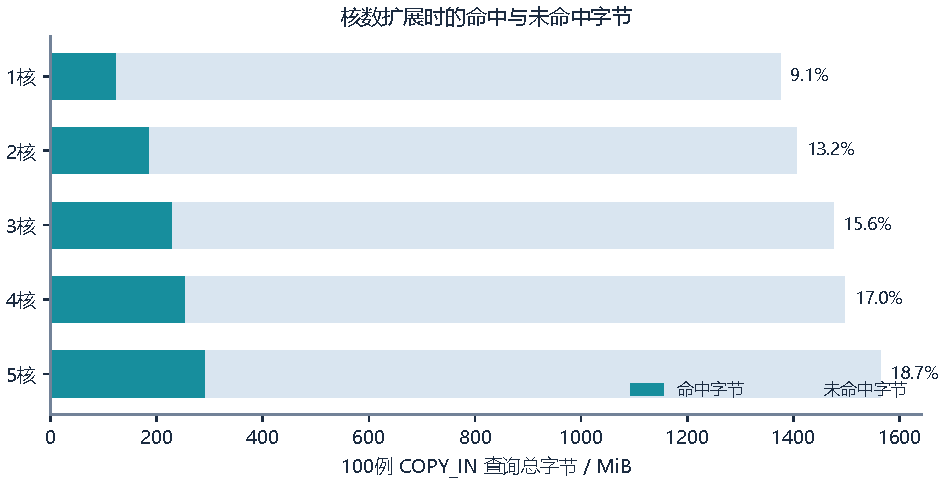
\includegraphics[width=160mm]{../求解/正式图件/q3-F05.pdf}
\caption{核数与L2查询字节}\label{fig:q3-f05}
\end{figure}

% Generated model comparison; edit scientific report and rerun the builder.
\noindent 本问是有显式约束和官方仿真目标的计算图组合优化；100 个图不提供最优方案标签，直接评价候选方案可复核，学习模型没有可验证的训练目标。\par


\subsection{逐核成对收益与命中含义}

Cache收益的正式统计必须把方案身份固定。对每个案例、核数先取问题三正式选中的$p$，分别在题定场景B无L2和有L2条件下评估$T^{(0)}(p)$、$T^{(L2)}(p)$，再形成逐例比值$R=T^{(0)}(p)/T^{(L2)}(p)$。表~\ref{tab:q3-core-deep}列出的均值是100个$R$的算术平均，而不是两个100例平均完成周期之比。两个汇总顺序不同：长图可能在平均周期中占主要权重，却在逐例比值平均中与短图各占一票。本文采用逐例求比的口径与原题加速比要求一致，因此不能用总命中字节数或总节约周期除以总时长代替。

\begin{table}[htbp]\centering
\caption{固定同一方案时的逐核L2收益分布}\label{tab:q3-core-deep}
\small\begin{tabular}{rrrrrr}\toprule
核数 & Cache比均值 & 中位数 & 受益/逆向例数 & 零命中例数 & 平均命中率 \\ \midrule
1 & 1.0086 & 1.0000 & 25/0 & 69 & 9.20\% \\
2 & 1.0120 & 1.0000 & 38/0 & 33 & 14.03\% \\
3 & 1.0143 & 1.0000 & 39/0 & 28 & 19.10\% \\
4 & 1.0190 & 1.0000 & 44/0 & 30 & 17.88\% \\
5 & 1.0260 & 1.0001 & 58/1 & 24 & 21.29\% \\
\bottomrule\end{tabular}\end{table}


从一核到五核，平均同方案收益依次为$1.0086$、$1.0120$、$1.0143$、$1.0190$、$1.0260$；严格受益案例数分别为25、38、39、44、58。这个趋势与图~\ref{fig:q3-f06}中两条平均加速比曲线的间距增大一致，但它们不是同一统计量：图~\ref{fig:q3-f06}分别对两种情景的$T_1/T_k$取均值，表中的收益则对同方案$T_k^{(0)}/T_k^{(L2)}$取均值。不同核数的方案本身会重新择优，因此从一核到五核的变化也不应被解释成“仅增加核心必然提高某张图的L2命中”。四核平均命中率$17.88\%$还低于三核的$19.10\%$，正说明不同分配、不同COPY访问序列会改变FIFO状态。

五核有24例命中字节率为零；在其余76例中，58例同方案时长改善，17例在记录精度下完全持平，1例出现极小的逆向差异。因而“有命中”既不是严格收益的充分条件，也不保证收益幅度与命中率成比例。计入命中率的字节可能属于非控制最后完工时刻的COPY，也可能与其它Pipe上的工作并行；从DDR转向Cache的读请求还会改变两个独立带宽池的排队与完成先后。算例002的$0.99995$是官方确定性事件模型中的三周期差异，不宜放大为稳定的硬件退化规律。反过来，算例083的$1.4240$也不能推广成“约68\%命中率通常带来42\%提速”，因为其它案例的依赖链与带宽竞争不同。

方案适配与缓存机制仍应分开评价。五核问题二与问题三的胜出候选族仅在1个案例不同，四核也仅在1个案例不同；这说明当前三种候选在默认L2配置下通常保留相同的胜出族，但“族名相同”不保证方案逐字节相同。因此本文在每一例的缓存收益分子、分母上固定问题三的实际方案，而没有假定问题二结果天然可作同方案对照。后续若扩大候选空间或改变Cache容量，候选切换次数都可能变化，必须重新进行这一成对评估。

\subsection{命中率分层的反例与统计边界}

图~\ref{fig:q3-f02}展示命中率与收益的联合形状；为核对离散点代表多少案例，表~\ref{tab:q3-hit-crosscheck}把正式五核的100例按命中字节率$H$分为四个互斥区间，并在每层重算同方案Cache比。分层阈值只是解释用途，不参与方案择优，也不是从网格敏感性实验中调出的参数。四层计数24、25、37、14之和恰为100。表中的“严格受益”按官方记录比值大于1计数，因而极小但真实的周期差异仍按其方向记录，不能把这一计数解释为统计显著性检验。

\begin{table}[htbp]\centering
\caption{五核命中字节率分层后的同方案收益}\label{tab:q3-hit-crosscheck}
\small\begin{tabular}{lrrrr}\toprule
命中字节率范围 & 例数 & Cache比均值 & 严格受益例数 & 最大Cache比 \\ \midrule
零命中 & 24 & 1.0000 & 0 & 1.0000 \\
$0<H\leq0.20$ & 25 & 1.0043 & 13 & 1.0642 \\
$0.20<H\leq0.50$ & 37 & 1.0459 & 31 & 1.2912 \\
$H>0.50$ & 14 & 1.0563 & 14 & 1.4240 \\
\bottomrule\end{tabular}\end{table}


零命中层的24例全部没有同方案时长收益，符合只读L2没有实际服务字节时的机制预期。低命中层$0<H\leq0.20$的25例中，仅13例严格受益，平均收益比$1.0043$；其余12例的COPY命中并未改变全局最后完成时刻。在$0.20<H\leq0.50$的37例中，31例受益，均值$1.0459$；高于$0.50$的14例全部受益，但均值也仅$1.0563$。各层平均值随命中率上升，是这100例的描述性关联；表内同层最大收益分别为$1.0642$、$1.2912$与$1.4240$，跨度显示命中率相近的图仍可能有很不同的时间收益。

具体而言，命中字节率的分子是成功由L2读出的总字节，不记录这些COPY位于哪条控制全局终点的依赖链，也不记录命中发生时DDR是否拥塞。用$H$预测时间至少还要知道命中读的事件位置、L2池占用、DDR池占用和与计算Pipe的重叠；本研究没有从汇总命中率逆推出这些不可观测的事件结构。高命中层14例全部改善不意味着“$H>0.50$是充分条件”，因为这个说法只在当前有限案例与给定配置下成立，换容量、带宽或FIFO访问次序就可能改变。表~\ref{tab:q3-hit-crosscheck}因此作为模型解释与反例核查，不能作为新的参数优化器。

\subsection{图结构与共享缓存收益的交叉核查}

问题一已经按最大弱连通块所占非COPY操作比例$f$划分四个结构组。为检验“容易切开的图是否一定更受益于共享L2”，本文沿用那四个预先使用的分界，而不根据缓存结果重新寻找最显著阈值；在每个组内只取官方五核的对应案例，分别计算逐例命中字节率和同方案收益比的算术平均。表~\ref{tab:q3-structure-cache}的四组人数为38、21、13、28，恰好覆盖正式100例，严格受益数加总为58，与不分组的原始统计一致。这种交叉核对也防止因结构分组遗漏案例而把小样本均值误作整体结论。

\begin{table}[htbp]\centering
\caption{五核图结构分组下的同方案Cache收益}\label{tab:q3-structure-cache}
\small
\begin{tabular}{c r r r r}
\toprule
最大连通块占比 & 案例数 & 平均命中字节率 & 平均收益比 & 严格受益数 \\
\midrule
$f\leq0.05$ & 38 & 24.48\% & 1.0279 & 20 \\
$0.05<f\leq0.20$ & 21 & 24.69\% & 1.0516 & 12 \\
$0.20<f\leq0.60$ & 13 & 22.71\% & 1.0244 & 9 \\
$f>0.60$ & 28 & 13.76\% & 1.0048 & 17 \\
\bottomrule
\end{tabular}
\end{table}


最大连通块占比大于$0.60$的28例，平均命中字节率为$13.76\%$、同方案收益比为$1.0048$；最分散的$f\leq0.05$组对应$24.48\%$和$1.0279$。在本组数据中，较分散的结构确实伴随较高的平均命中与收益，但它并不构成单调的性能定律：$0.05<f\leq0.20$组的平均收益$1.0516$高于最分散组的$1.0279$，两组平均命中率却十分接近。中间的$0.20<f\leq0.60$组也不能仅按$f$在两端之间插值推算；它只有13例，均值容易受个别图的访问路径影响。

组内正向案例数进一步揭示均值的限制。$f>0.60$组仍有17/28例严格受益，说明较大的连通块不等于共享输入完全没有重用；只是这些改善的总平均幅度较小。$f\leq0.05$组虽然平均收益较高，严格受益也只有20/38例，其中算例083的同方案比值达到$1.4240$，使组内分布出现明显右尾。若用一个结构阈值直接决定是否开启L2，既会错过高连通组中的实际受益图，也会把低连通但处于非关键读链的图误判为高收益。$f$刻画图能否按弱连通成分拆开，$H$刻画产生了多少命中字节，$R$才是完整事件时间线的结果；三者的层级不能互相替代。

上述关联还受到候选择优的条件化影响：各组在五核下使用的切图候选可能不同，改变跨核输入复用和COPY访问次序。表内每个$R$的分子分母仍固定同一问题三方案，所以缓存收益的成对定义未变，但跨组比较并未固定方案族，也未控制图规模、深度与原始COPY强度。它只能说明当前100例的结构异质性，不能把最大连通块占比解释为对Cache收益的独立因果作用。后续若要建立可迁移的收益预测器，需要在同一图上对多个候选与多个容量配置做成组评价，并保留关键读事件和FIFO状态轨迹；本文没有用现有汇总表冒充这些尚未完成的实验。

\subsection{参数敏感性与独立核验}

为考察参数响应，另取6例有代表性的正式五核图，在复制的配置上设置容量$256\,\mathrm{KiB}$、$1\,\mathrm{MiB}$、$4\,\mathrm{MiB}$与读带宽$60,250,500$字节每周期的九格组合。每格重新评估全部可用候选，共54条最优记录；默认$1\,\mathrm{MiB}/250$格同正式实验逐字节复核一致。所有参数变化均为非官方配置，没有混入题定100例成绩。

图~\ref{fig:q3-f03}给出案例044与083的实测三维响应面，图中高度刻度以千周期为单位。044在该网格的完成周期范围为$98948$至$132892$，083为$287606$至$442480$；响应并不平坦。三维表面只连接九个实际网格点，不能解释为连续空间中的已验证插值最优。图~\ref{fig:q3-f04}在固定读带宽250字节每周期时，对照六例容量变化下的命中字节率；它展示缓存状态的响应，不直接展示完成周期。再从九格结果读取时长：在默认容量下将带宽从250提高到500，044的完成时间比为$1.0402$，083为$1.0684$；在默认带宽下把容量从1MiB提高至4MiB，044没有可测改善，083改善约$0.91\%$。这说明命中率和完工时间属于不同层次的结果，参数响应不能由单一全局命中率预测。

\begin{figure}[htbp]\centering
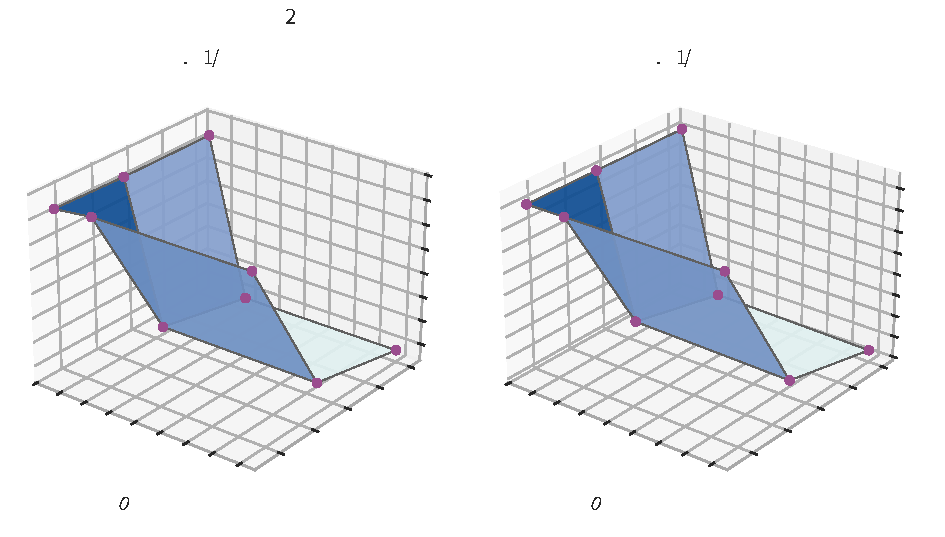
\includegraphics[width=160mm]{../求解/正式图件/q3-F03.pdf}
\caption{非官方L2参数响应面}\label{fig:q3-f03}
\end{figure}

\begin{figure}[htbp]\centering
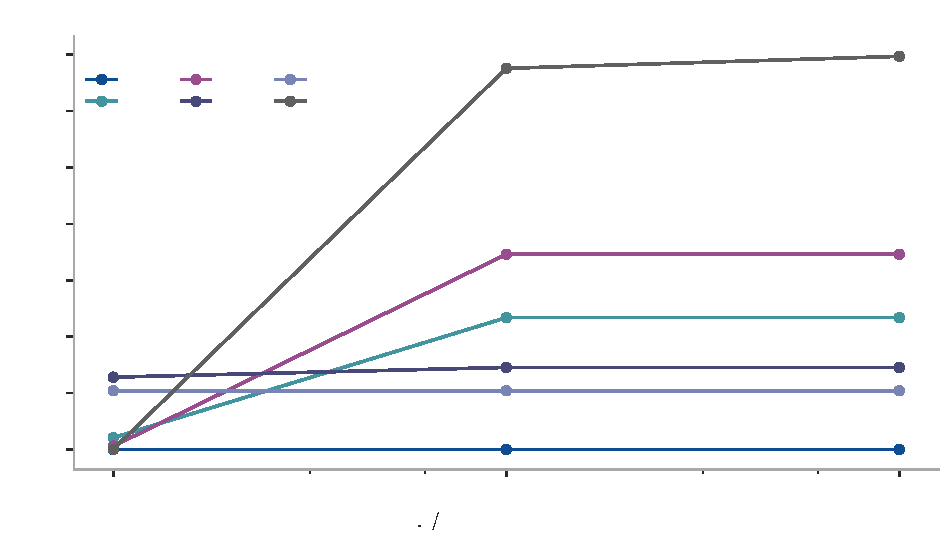
\includegraphics[width=160mm]{../求解/正式图件/q3-F04.pdf}
\caption{固定带宽下的容量与命中率响应}\label{fig:q3-f04}
\end{figure}

\subsection{有限网格内的条件差分}

为免把非官方网格误写成连续寻优，表~\ref{tab:q3-grid-deep}只在实际评价过的九个格点做有限差分。每一行的默认点是容量$1$ MiB、读带宽$250$字节每周期；“容量增益”指只把容量改到$4$ MiB时默认周期减少的百分比，“带宽增益”指只把读带宽改到$500$字节每周期时减少的百分比，均以本行默认周期为分母。表内还给出该案例九格完成时间的最小值和最大值，但区间端点未必来自同一参数轴，因此不可把“范围”当作某个单参数的因果效应。

\begin{table}[htbp]\centering
\caption{六例非官方L2网格在默认点附近的有限差分}\label{tab:q3-grid-deep}
\small\begin{tabular}{lrrrr}\toprule
算例 & 默认周期 & 九格范围/千周期 & 容量增益 & 带宽增益 \\ \midrule
001 & 47502 & 47.5--47.5 & 0.00\% & 0.00\% \\
002 & 55099 & 55.1--55.1 & 0.00\% & 0.00\% \\
044 & 102921 & 98.9--132.9 & 0.00\% & 3.86\% \\
050 & 84038 & 84.0--84.0 & 0.00\% & 0.00\% \\
056 & 219072 & 219.1--219.1 & 0.00\% & 0.00\% \\
083 & 310731 & 287.6--442.5 & 0.90\% & 6.40\% \\
\bottomrule\end{tabular}\end{table}


六例的响应强弱差别很大。算例001在九格中全部是$47502$周期，默认命中字节率为零；读带宽或容量在本次格点内改变，自然不会从这份记录产生可测收益。算例056虽有约$10.43\%$的默认命中率，九格也全部保持$219072$周期，说明其被L2服务的读在本评估范围内没有改变最后完成事件。算例002九格只跨$55099$至$55108$周期，算例050只跨$84036$至$84047$周期；相对于各自的总时长，这些变化极小。不能仅凭命中比例把这些案例排列成统一的性能响应顺序。

算例044和083构成另一端。044九格范围为$98948$至$132892$周期，在默认容量下提高带宽至$500$时完成时间降低$3.86\%$，而默认带宽下把容量增到$4$ MiB没有可测改善。083九格范围为$287606$至$442480$周期，带宽增益为$6.40\%$，容量增益为$0.90\%$；从默认带宽$250$反向降至$60$，在默认容量下其完成时间增加约$42.40\%$，044对应增加约$29.12\%$。这些数值揭示在当前两张图的固定方案和九格范围内，读带宽限制比容量增加更明显；然而其它四例并不呈现同样强的响应，故不对100例作平均参数结论。

该六例由正式结果的不同收益层选取，目的在覆盖机制表现，而不是对全体算例作随机抽样。每格既评估固定默认方案，也重新比较可用候选；在当前六例九格中，胜出候选族均没有切换，所以表~\ref{tab:q3-grid-deep}的时长变化主要对应参数路径而非候选族更换。仍需注意同族方案的具体排程在其它配置上可能改变，且格点之间没有额外试验，三维图面只供观察九点相邻关系。若将来增加容量或带宽范围、引入其它候选，必须重新检查默认格身份、候选切换以及官方与独立核验的一致性。把这一非官方实验与题定默认100例分开记录，是本文控制外推范围的必要条件。

独立程序逐格核对候选记录、配置副本和官方响应，54格统计审计通过；所选五百组方案的覆盖、时间线及官方响应交叉核验全部通过。共享L2只服务只读COPY\_IN，写回流量、私有缓存容量和无法共享的张量仍限制加速；本研究没有实测芯片功耗与物理时延，结论限定在题目给定的事件评估模型。





\GMCMChapterEnd{6}
\section{模型评价与展望}
\subsection{模型优点}

\begin{enumerate}
\item \textbf{优点一：以官方全局完成时间闭合建模与求解。} 三问都把切图、同核顺序、跨核依赖和存储行为落实为可执行方案，再由题定评估器计算 Makespan。候选的粗负载、连通块大小或命中字节率只是构造和诊断量，不被误写成实际完成时间。问题一的五核平均加速比为$3.5093$，问题二为$3.5456$，问题三为$3.6104$；这些数值均来自100个官方算例的完整配置，而非代理目标的预测。

\item \textbf{优点二：使用成对反事实分离场景与缓存机制。} 问题二把问题一的同一方案重新放入场景B，先测量Task合并、私有存储驻留与COPY规则改变的净影响，再与场景B重新择优的附加收益区分。问题三在相同算例、核数、切图和同核顺序上比较无L2与题定L2评估结果，使场景差异与候选更替不混入Cache机制收益。逐例比例而非只有总均值保留了有益、无益和不利的真实差异。

\item \textbf{优点三：保留可追溯的方案、响应和独立复核。} 对100例与五种核数逐一保存方案、官方原始响应和结构化摘要；问题一至问题三所选配置各有500份独立检查记录。校验覆盖操作唯一性、子图依赖、同核顺序及关键时间线，减少将评估器成功退出误当作科学验证的风险。候选失败也被保留在模型比较记录中，不用缺失分数冒充劣势。

\item \textbf{优点四：把结构异质性纳入解释。} 输入图的弱连通块与宽度差异决定连通块、深度分段和分批候选的适用范围；正式结果同时报告分位数、逐例非单调性与候选胜出频数。这样，平均加速比之外的低收益尾部及新增DDR搬运都能与调度机制对应，而不被单一汇总指标掩盖。
\end{enumerate}

\subsection{模型缺点}

\begin{enumerate}
\item \textbf{缺点一：有限候选集不保证全局最优。} 方案只在预先确定的连通块、八段深度划分和宽图分批三类候选中择优，没有穷举合法切图与核内顺序。特别是较大的弱连通块若需要非均匀切分，固定深度段可能错过更好的并行安排。因此文中加速比是可复核的可行结果，不能宣称达到理论最优。

\item \textbf{缺点二：粗负载未精确预报资源争用。} 连通块权重主要汇总操作计算周期，对共享DDR带宽、四条Pipe、固定Task等待及L1/UB容量的联合作用没有建立闭式代理。它足以产生合法候选，却可能把局部均衡方案送入全局拥塞；正式结果中随核数增加仍出现逐例速度下降，说明代理与Makespan之间存在结构依赖。

\item \textbf{缺点三：问题三的参数外推范围有限。} 正式成绩只对应题定L2容量和带宽。另选六个结构不同的算例做54格容量—带宽网格，是解释命中和瓶颈的非官方机制实验，并非官方100例的重新计分。网格中候选身份保持不变，能帮助隔离参数影响，却不能代表所有算例在其他硬件配置下的最优策略。

\item \textbf{缺点四：模型依赖题给评估语义。} FIFO不刷新次序、COPY\_IN按逻辑张量编号查询和两条读带宽池等规则都按官方实现核验。真实处理器若增加写回、异步预取、不同缓存一致性或变动的Task启动成本，原候选排序可能改变，须重新标定而不能直接套用本文速度比。
\end{enumerate}

\subsection{模型的推广与改进}

这套“依赖图切分—可执行方案—事件评估—成对反事实”的程序可用于具有明确操作依赖、可配置并行执行资源和可观察搬运成本的其他推理或数据流处理器。推广的前提是准确重建目标设备的合法性规则、存储层级、Pipe并发与固定开销，并提供与之匹配的评估或实机计时接口。若只有粗略峰值算力而缺少资源争用数据，本文的方案生成思想仍可借用，但不能迁移本文的数值加速结论。

针对有限候选集，后续可在保持覆盖与无环约束的前提下，对大连通块增加按关键路径、边界张量字节和容量余量联合引导的自适应切分；对已有方案实施局部合并、迁核和同核重排。每次改动应在固定案例划分和相同官方评估预算下成对比较，同时报告改进幅度与额外计算成本。针对缓存参数，宜扩大结构分层抽样，并在不同容量与带宽上重新优化候选，与同方案机制反事实分别报告；只有当独立复核和完整输入范围保持成立，才可将其作为新的正式策略。

\GMCMChapterEnd{7}
\clearpage
\begin{thebibliography}{99}
\bibitem{sze2017} Sze V, Chen Y H, Yang T J, Emer J S. Efficient Processing of Deep Neural Networks: A Tutorial and Survey. Proceedings of the IEEE, 105(12): 2295--2329, 2017.
\bibitem{eyeriss2017} Chen Y H, Krishna T, Emer J S, Sze V. Eyeriss: An Energy-Efficient Reconfigurable Accelerator for Deep Convolutional Neural Networks. IEEE Journal of Solid-State Circuits, 52(1): 127--138, 2017.
\bibitem{jouppi2017} Jouppi N P, Young C, Patil N, et al. In-Datacenter Performance Analysis of a Tensor Processing Unit. Proceedings of the 44th Annual International Symposium on Computer Architecture, 1--12, 2017.
\bibitem{hongkung1981} Hong J W, Kung H T. I/O Complexity: The Red-Blue Pebble Game. STOC 1981: 326--333, 1981.
\bibitem{perotin2021} Perotin L, Sun H, Raghavan P. Multi-Resource List Scheduling of Moldable Parallel Jobs under Precedence Constraints. arXiv:2106.07059, 2021.
\bibitem{topcuoglu2002} Topcuoglu H, Hariri S, Wu M Y. Performance-Effective and Low-Complexity Task Scheduling for Heterogeneous Computing. IEEE Transactions on Parallel and Distributed Systems, 13(3): 260--274, 2002.
\bibitem{kernighan1970} Kernighan B W, Lin S. An Efficient Heuristic Procedure for Partitioning Graphs. Bell System Technical Journal, 49(2): 291--307, 1970.
\bibitem{karypis1998} Karypis G, Kumar V. A Fast and High Quality Multilevel Scheme for Partitioning Irregular Graphs. SIAM Journal on Scientific Computing, 20(1): 359--392, 1998.
\bibitem{chen2018tvm} Chen T, Moreau T, Jiang Z, et al. TVM: An Automated End-to-End Optimizing Compiler for Deep Learning. 13th USENIX Symposium on Operating Systems Design and Implementation (OSDI 18), 578--594, 2018.
\bibitem{mattson1970} Mattson R L, Gecsei J, Slutz D R, Traiger I L. Evaluation Techniques for Storage Hierarchies. IBM Systems Journal, 9(2): 78--117, 1970.
\end{thebibliography}

\GMCMChapterEnd{8}
\clearpage
% Generated by tools/build_appendix.py; do not hand-edit.
% Styling is owned exclusively by 章节模板/附录模板.tex.
\AppendixStart
\AppendixPart{1}{附件文件及内容}
\AppendixAttachmentTableBegin
\AppendixAttachmentRow{1}{问题一}{场景A切图与调度源码、逐例官方结果及候选比较}
\AppendixAttachmentRow{2}{问题二}{场景B同核Task合并源码、成对对照及候选比较}
\AppendixAttachmentRow{3}{问题三}{共享只读L2调度源码、缓存收益及非官方敏感性表}
\AppendixAttachmentRow{4}{其他数据}{题目原始100图与固定配置归档}
\AppendixAttachmentRow{5}{其他支撑材料}{全部正式候选响应、逐例指标、汇总及非官方网格核验}
\AppendixAttachmentTableEnd
\AppendixPart{2}{问题一关键代码}
\AppendixCodeFile[firstline=1,lastline=9,firstnumber=1]{本问唯一复现入口（片段 1）}{python}{../求解/问题一/问题一.py}
\AppendixCodeFile[firstline=58,lastline=170,firstnumber=58]{题目提供且未改动的官方评估源码（片段 2）}{python}{../数据/原始/A题官方附件/code/contest_io.py}
\AppendixCodeFile[firstline=195,lastline=293,firstnumber=195]{题目提供且未改动的官方评估源码（片段 3）}{python}{../数据/原始/A题官方附件/code/contest_io.py}
\AppendixCodeFile[firstline=20,lastline=24,firstnumber=20]{题目提供且未改动的官方评估源码（片段 4）}{python}{../数据/原始/A题官方附件/code/evaluation_validation.py}
\AppendixCodeFile[firstline=106,lastline=111,firstnumber=106]{题目提供且未改动的官方评估源码（片段 5）}{python}{../数据/原始/A题官方附件/code/evaluation_validation.py}
\AppendixCodeFile[firstline=171,lastline=243,firstnumber=171]{题目提供且未改动的官方评估源码（片段 6）}{python}{../数据/原始/A题官方附件/code/evaluation_validation.py}
\AppendixCodeFile[firstline=200,lastline=214,firstnumber=200]{题目提供且未改动的官方评估源码（片段 7）}{python}{../数据/原始/A题官方附件/code/multicore_cut_evaluate_problem_1.py}
\AppendixPart{3}{问题二关键代码}
\AppendixCodeFile[firstline=1,lastline=9,firstnumber=1]{本问唯一复现入口（片段 1）}{python}{../求解/问题二/问题二.py}
\AppendixCodeFile[firstline=58,lastline=170,firstnumber=58]{题目提供且未改动的官方评估源码（片段 2）}{python}{../数据/原始/A题官方附件/code/contest_io.py}
\AppendixCodeFile[firstline=195,lastline=293,firstnumber=195]{题目提供且未改动的官方评估源码（片段 3）}{python}{../数据/原始/A题官方附件/code/contest_io.py}
\AppendixCodeFile[firstline=20,lastline=24,firstnumber=20]{题目提供且未改动的官方评估源码（片段 4）}{python}{../数据/原始/A题官方附件/code/evaluation_validation.py}
\AppendixCodeFile[firstline=106,lastline=111,firstnumber=106]{题目提供且未改动的官方评估源码（片段 5）}{python}{../数据/原始/A题官方附件/code/evaluation_validation.py}
\AppendixCodeFile[firstline=171,lastline=243,firstnumber=171]{题目提供且未改动的官方评估源码（片段 6）}{python}{../数据/原始/A题官方附件/code/evaluation_validation.py}
\AppendixCodeFile[firstline=200,lastline=214,firstnumber=200]{题目提供且未改动的官方评估源码（片段 7）}{python}{../数据/原始/A题官方附件/code/multicore_cut_evaluate_problem_1.py}
\AppendixPart{4}{问题三关键代码}
\AppendixCodeFile[firstline=1,lastline=9,firstnumber=1]{本问唯一复现入口（片段 1）}{python}{../求解/问题三/问题三.py}
\AppendixCodeFile[firstline=58,lastline=170,firstnumber=58]{题目提供且未改动的官方评估源码（片段 2）}{python}{../数据/原始/A题官方附件/code/contest_io.py}
\AppendixCodeFile[firstline=195,lastline=293,firstnumber=195]{题目提供且未改动的官方评估源码（片段 3）}{python}{../数据/原始/A题官方附件/code/contest_io.py}
\AppendixCodeFile[firstline=20,lastline=24,firstnumber=20]{题目提供且未改动的官方评估源码（片段 4）}{python}{../数据/原始/A题官方附件/code/evaluation_validation.py}
\AppendixCodeFile[firstline=106,lastline=111,firstnumber=106]{题目提供且未改动的官方评估源码（片段 5）}{python}{../数据/原始/A题官方附件/code/evaluation_validation.py}
\AppendixCodeFile[firstline=171,lastline=243,firstnumber=171]{题目提供且未改动的官方评估源码（片段 6）}{python}{../数据/原始/A题官方附件/code/evaluation_validation.py}
\AppendixCodeFile[firstline=200,lastline=214,firstnumber=200]{题目提供且未改动的官方评估源码（片段 7）}{python}{../数据/原始/A题官方附件/code/multicore_cut_evaluate_problem_1.py}
\AppendixEnd

\end{document}
